\documentclass{article}
\usepackage[english]{babel}
%\usepackage[utf8x]{inputenc}
%\usepackage{apacite}
\usepackage[toc,page]{appendix}
%\usepackage{biblatex} % place in the document preamble
%%---------- path ------------%%
%\def\input@path{{~/Dropbox/6_Graduate/}}
%%---------- my command --- ----------%%
\newcommand{\pard[1]}{\frac{\partial}{\partial{#1}}}
\newcommand{\mean[1]}{\frac{1}{n}\sum_{i=1}^{#1}}
\newcommand{\defeq}{\vcentcolon=}
\newcommand{\eqdef}{=\vcentcolon}
\newcommand\independent{\protect\mathpalette{\protect\independenT}{\perp}}
\newcommand{\wh}{\widehat}
\newcommand{\itl}{\intercal}
\newcommand{\p}{\prime}
\newcommand{\bs}{ \boldsymbol}
\newcommand{\mb}{\mathbb}
\newcommand{\ml}{\mathcal}
\newcommand{\br}{\bar}
\newcommand{\txt}{\text}
\newcommand{\lt}{\left}
\newcommand{\rt}{\right}
\newcommand{\lv}{\lvert}
\newcommand{\rv}{\rvert}
\newcommand{\nlim}{\underset{n \to \infty}{\lim}}
\newcommand{\smb}{\begin{bmatrix}}
	\newcommand{\sme}{\end{bmatrix}}
\newcommand\indep{\protect\mathpalette{\protect\independenT}{\perp}}
\def\independenT#1#2{\mathrel{\rlap{$#1#2$}\mkern2mu{#1#2}}}
\newcommand{\tsgn}{\txt{sgn}}


%%-------- my package -------%%
\usepackage{ragged2e}
\usepackage{float}
\usepackage{epstopdf}
\usepackage[final]{pdfpages}
%\usepackage{cite}
\usepackage{amsmath}
\usepackage{color}
\usepackage{graphicx}
\usepackage{verbatim}
\usepackage{commath}
\usepackage{caption}
%\usepackage{bbm}
%\usepackage{xfrac}
%\usepackage{dsfont}
\usepackage{amssymb}
\usepackage{verbatim}
\usepackage{mathtools}
\usepackage{resizegather}
\usepackage{xfrac}
\usepackage{amsthm}
\usepackage[ruled]{algorithm2e}
%\newtheorem{remark}{Remark}
%\newtheorem{lemma}{Lemma}
%\newtheorem{theorem}{Theorem}
%\newtheorem{corollary}{Corollary}
\newtheorem{theorem}{Theorem}[section]
\newtheorem{lemma}[theorem]{Lemma}
\newtheorem{proposition}[theorem]{Proposition}
\newtheorem{corollary}[theorem]{Corollary}
\renewcommand\qedsymbol{$\blacksquare$}

%%----------------------------------------------------------------------------%%
%%------------------------------ Import Packages -----------------------------%%
%%----------------------------------------------------------------------------%%


\usepackage{booktabs}  % professionally typeset tables
\usepackage{amsmath}
\usepackage{textcomp}  % better copyright sign, among other things
\usepackage{xcolor}
\usepackage{lipsum}    % filler text
\usepackage{subfig}    % composite figures


%%----------------------------------------------------------------------------%%
%%---------------------------- Formatting Options ----------------------------%%
%%----------------------------------------------------------------------------%%
%%

%% -------------------------------------------------------------------------- %%
%% Disposition format -- any titles, headings, section titles
%%  These formatting commands affect all headings, titles, headings,
%%  so sizing commands should not be used here.
%%  Formatting options to consider are
%%     +  \sffamily - sans serif fonts.  Dispositions are often typeset in
%%                    sans serif, so this is a good option. 
%%     +  \rmfamily - serif fonts
%%     +  \bfseries - bold face
%\dispositionformat{\sffamily\bfseries}   % bold and sans serif


%% ------------------------------
\title{Constrained Estimation of Single-stage Optimal Treatment Regimes}
\author{Shuping Ruan, Eric Laber\\ Department of Statistics, North Carolina State University}


\begin{document}
\maketitle

\section{Introduction}
Precision medicine aims to accommodate interventions to individual patient attributes. For chronic illnesses, such as cancer, diabetes and so on, clinicians often need to make sequences of treatment decisions based on the evolving status of the patient's condition. To personalize this multi-stage intervention process, researchers have been developing dynamic treatment regimes (DTRs) to inform clinicians of treatment decisions adaptively. DTRs are a sequential decision making process, of which each decision is made based on the evolving patient status with the goal of maximizing the overall long-term treatment efficacy. It is well-studied in the statistical and biomedical literature ~\cite{Murphy2003, Moodie2004,Murphy2005,Zhang2012, Laber2014,Linn2014}. From the standpoint of Markov decision process, reinforcement learning algorithms, such as Q-learning~\cite{Murphy2005}, A-learning~\cite{blatt2004learning}, V-learning~\cite{Luckett2016} etc., are developed to estimate optimal treatment regimes. \\

Most previous methods for construct optimal dynamic treatment regimes have focused on optimizing a scalar measurement of the long-term efficacy over a fixed time period (finite stage).  However, in practice, the clinical situations are more complex. First, they often require consideration of the trade-off among multiple objectives, e.g., effectiveness, side-effect, cost, and so on. The preference of those objectives varies among people and changes over time, thus a single scalar reward or value can not represent the quality of a policy well enough. Thus, considering multiple rewards are necessary. Previous works by Lizotte et al. learn the value function and optimal policy for all preferences, i.e., all the possible convex combination of all the rewards~\cite{Lizotte2010,Lizotte2012}. More recent works adopt multi-objective Markov decision processes (MOMDPs) framework with finite stage. Practical domination is proposed for flexibility based on Pareto domination, and a set of policies that are maximal based on the partial order are treated as indistinguishably optimal~\cite{LaberTwo2014, Lizotte2016}. Secondly, patients with chronic diseases are often monitored and treated throughout their life. It often requires taking real-time actions and has no a-priori fixed end point (infinite stage), and progress is made in infinite stage reinforcement learning for health applications~\cite{Ertefaie2014,Murphy2016,Luckett2016}.\\

To deal with the trade-off between multiple objectives, we take a different perspective and adopt the constrained Markov decision processes (CMDPs) framework with infinite horizon. CMDPs are a well-studied framework for reinforcement learning under constraints~\cite{altman99cmdp}. The goal is to find the optimal policy, while satisfying constraints on expectations of secondary costs. For many applications of reinforcement learning, the constrained approach is more intuitive and more practical than eliciting a single reward function in order to achieve desirable results. For instance, satisfying safety constraints is necessary for systems that physically interact with humans. Previously, linear programming is used to seek constrained optimal policies in the setting of finite CMDPs with known models. However, few methods have been proposed for high-dimensional constrained reinforcement learning problems without modeling the underlying dynamics. Recently, Achiam et al~\cite{Achiam2017} proposed constrained policy optimization, a general-purpose policy search algorithm for constrained reinforcement learning guaranteeing near-constraint satisfaction at each iteration. Taking into consideration properties of clinical applications, such as data scarcity and off-policy learning, we develop an algorithm by taking advantage of least-squares policy evaluation and interior-point methods for estimating constrained optimal dynamic treatment regimes. Our method is applied to a simulated cancer trial dataset based on a chemotherapy mathematical model.\\

\section{Methodology}
\subsection{Set-up}
\subsubsection*{Observed Data}
We use dataset observed over a finite length of time steps to construct a regime in the setting of infinite horizon Markov decision process. The structure of the available data is  $\bs{D} = \lt\{  (\bs{S}^i_{0}, A^i_{0}, \bs{R}^i_{0} , \bs{S}^i_{1}, \cdots, 
\bs{S}^i_{T_i-1} , A^i_{T_i-1}, \bs{R}^i_{T_i-1}, \bs{S}^i_{T_i}) \rt\}_{i=1}^n,$
a set of $n$ independent, identically distributed trajectories of\\
$\lt(\bs{S}_{0}, A_{0}, \bs{R}_{0} , \bs{S}_{1}, \cdots, 
\bs{S}_{T-1} , A_{T-1}, \bs{R}_{T-1}, \bs{S}_{T}\rt).$
Note $T \in \mb{N}$ denotes the total number of follow-up time steps for a patient. For each patient, his or her follow up time length $T_i$ may be different. $\bs{S}_{t} \in \bs{\ml{S}}$ denotes a vector of patient clinical information recorded up to and including time point $t$, referred as \textit{state} in the reinforcement learning vocabulary. $\bs{\ml{S}} \subseteq \mb{R}^m$ denotes the support for state variable. Adopting the time homogeneous Markov decision process model, we assume $\bs{\ml{S}}$ is the same across all time points $t$.  $A_{t} \in \ml{A}$ denotes the treatment assignment at time point $t$ after measuring $\bs{S}_{t},$  referred as \textit{action} in reinforcement learning.  $\ml{A}$ denotes the support for treatment assignment, a finite set of all possible treatment options, and is assumed to be the same across all time points $t$. $\bs{R}_{t} \in \mb{R}^J$ is the reward obtained after treatment $A_{t}$ is assigned. We assume the reward, possibly defined based on domain expertise, is a known vector-valued function $\bs{r}$: $\bs{\ml{S}} \times \ml{A}  \times \bs{\ml{S}} \to \mb{R}^J $, so that $\bs{R}_{t} = \bs{r}(\bs{S}_{t}, A_t, \bs{S}_{t+1})$. The vector-valued reward function is the same across all the time points $t$ as well. Moreover, if a patient dies during the follow-up, say at decision point $t$, we set $\bs{S}_t = \bs{\emptyset}$, referred to as the absorbing state in reinforcement learning. Then, the patient's treatment assignment at time $t$ is $A_t=\emptyset$, and his/er length of follow-up $T = t$.	
\subsubsection*{Potential outcomes}
In reality, a patient can only be assigned to one of the sequences of treatment assignments. Hence, we can only observe the consequence of that treatment sequence, while the others remain unobserved. To identify the average causal effect of a certain regime, we adopt the counter-factual or potential outcomes framework,  established by Neyman, Rubin and Robins for assessment of the time-dependent treatment effect from either randomized or observational studies~\cite{Neyman,Robins1997,Rubin1980}. Let $\br{\bs{a}}_{t} = (a_0, a_1, \cdots, a_t) \in \br{\bs{\ml{A}}}_{t}$ be a possible treatment assignment sequence up to time point $t$, $t \ge 0$, where $\br{\bs{\ml{A}}}_t = \ml{A} \times \cdots \times \ml{A}$ is the set of all possible the treatment assignment sequences up to time point $t$. Let $\br{\bs{s}}_{t} = (\bs{s}_0, \bs{s}_1, \cdots, \bs{s}_t) \in \br{\bs{\ml{S}}}_{t}$ be a possible state sequences up to time point $t$, $t \ge 0$, where $\br{\bs{\ml{S}}}_t = \bs{\ml{S}} \times \cdots \times \bs{\ml{S}} $ is the set of all possible state sequences up to time point $t$. The set of potential outcomes is $\bs{W}^* = \lt\{\bs{S}^*_1(a_0), \bs{S}^*_2(\br{\bs{a}}_1),\cdots,  \bs{S}^*_{t+1}(\br{\bs{a}}_{t}), \cdots, \text{ for all } \br{\bs{a}}_{\infty} \in \br{\bs{\ml{A}}}_{\infty} \rt\}$, where $\bs{S}^*_{t+1}(\br{\bs{a}}_{t})$ is the potential state at $(t+1)$-th time point that would have been observed if the individual had been assigned the treatment sequence $\br{\bs{a}}_{t}$, $t \ge 0$. Moreover, if $\bs{S}_{t+1}^*(\br{\bs{a}}_{t}) = \bs{\emptyset}$ happens at time point $t+1$, then $\bs{S}_{t+2}^*(\br{\bs{a}}_{t+1}) =\bs{S}_{t+3}^*(\br{\bs{a}}_{t+2}) = \cdots = \bs{\emptyset}$, which indicates the patient, if followed treatment assignment sequence $\br{\bs{a}}_t$, would have died at time point $t+1$ in the counter-factual world.  Rewards with respect to potential states are $\bs{R}^*_t = \bs{r}(\bs{S}^*_t, A_t, \bs{S}^*_{t+1})$. The following assumptions are made in the potential outcome framework~\cite{Neyman, Rubin2005, Rubin1980, Robins1997, Hernan2006}.
\begin{itemize}
	\item  \textit{A1}. \textit{Consistency}:  $\bs{S}_{t+1} = \bs{S}^*_{t+1}(\br{\bs{A}}_{t})$, for all $t \ge 0$.
	\item \textit{A2}.  \textit{Sequential randomization assumption}: $A_{t+1} \indep \bs{W}^* \mid \br{\bs{S}}_{t+1}, \br{\bs{A}}_{t}$, for all $t \ge 0$.
	\item \textit{A3}. \textit{Positivity}: there exists $\epsilon_0 > 0$, so that $P\lt( A_{t+1} = a_{t+1} \mid \br{\bs{S}}_{t+1} = \br{\bs{s}}_{t+1}, \br{\bs{A}}_{t} = \br{\bs{a}}_{t} \rt) > \epsilon_0$, for all $a_{t+1} \in \mathcal{A}$, $\br{\bs{a}}_{t} \in \br{\bs{\ml{A}}}_t$ and $\br{\bs{s}}_{t+1} \in \br{\bs{\ml{S}}}_{t+1}$, and all $t \ge 0$.	 
\end{itemize}
These assumptions link the potential outcome and the observed data, and are guaranteed in well-designed Sequential, Multiple Assignment, Randomized Trials (SMARTs).  Therefore, the observed data from those trials are used to infer the average causal effect of a regime of interest.  

\subsubsection*{Markov Decision Processes}
To construct a regime in the infinite-horizon setting using a dataset observed over a finite number of time steps, we assume that the underlying dynamics is a time homogeneous Markov Decision Processes (MDPs). In infinite-horizon setting, MDP is considered as a 5-tuple of $(\bs{\ml{S}}, \ml{A}, \mb{P}, \bs{R}, \gamma)$, where $\bs{\ml{S}}$, $\ml{A}$ and $\bs{R}$ is as described above. Additionally, $\mb{P}$ is a markovian transition model in which $p(\bs{s}^{\prime} \mid \bs{s}, a)$ denotes the probability density of a transition to state $\bs{s}^{\prime}$ when taking action $a$ in state $\bs{s}$.  A discount factor for future reward, $\gamma \in [0, 1)$, is also introduced to form total discounted rewards, which are the value functions to operate constrained optimization on. The following assumptions are made for infinite-stage time homogeneous Markov decision process.
\begin{itemize}         
	\item \textit{A4}. \textit{Markov assumption}: $\bs{S}_{t+1} \indep \lt( \br{\bs{A}}_{t-1}, \br{\bs{S}}_{t-1} \rt) \mid \lt( A_{t}, \bs{S}_{t} \rt) $, for all $t \ge 1$.
	\item \textit{A5}. \textit{Time homogeneity}: the conditional density	$P_t(\bs{S}_{t+1} = \bs{s}^{\prime} \mid A_{t} = a, \bs{S}_{t} = \bs{s} ) = p(\bs{s}^{\prime} \mid a, \bs{s})$ for all $\bs{s} , \bs{s}^{\prime} \in \bs{\mathcal{S}}$ and $a \in \mathcal{A}$ and $t \ge 0$, where $\bs{s}$ and $\bs{s}^{\prime}$ denote the current state and the next state, respectively. 
\end{itemize}
As the time homogeneity is assumed in infinite-stage(3. setting, time step subscripts maybe dropped for simplicity.
\subsubsection*{Values of dynamic treatment regimes}
A dynamic treatment regime is equivalent to a \textit{policy} in reinforcement learning vocabulary, which is mostly to be considered deterministic. Thus, a dynamic treatment regime, $\pi : \bs{\ml{S}} \to \mathcal{A}$, is defined as a function which maps the support of the state variable to the set of the possible treatment assignments. As time homogeneity is assumed, we consider only stationary deterministic regimes, where this mapping function $\pi(\bs{s})$ does not change over time. Hence, a patient with state $\bs{S}_t = \bs{s}$ at time point $t$ will be assigned with treatment $A_t = \pi\lt(\bs{s}\rt)$ for all $t$.  
The value function $\bs{V}^{\pi}\lt(\bs{s}\rt)$ of a state under a certain policy $\pi$ is defined as the expected total discounted rewards when the process begins in state $\bs{s}$ and all decisions are made according to policy $\pi$. Mathematically, $\bs{V}^{\pi}\lt(\bs{s}\rt) = \mb{E}_{\bs{s}}^{\pi} \sum_{t=0}^{\infty} \gamma^{t} \, \bs{r}(\bs{s}_t, a_t, \bs{s}_{t+1})$, where $\mb{E}_{\bs{s}}^{\pi}$ is the expectation when the initial state is $\bs{s}$ and a policy $\pi$ is followed. The value function can also be defined recursively via the bellman equation, $\bs{V}^{\pi}\lt(\bs{s}\rt) = \sum_{\bs{s}^{\prime}\in\bs{\ml{S}}}  p(\bs{s}^{\prime} \mid \bs{s}, \pi(\bs{s})) \lt(\bs{R}(\bs{s}, \pi(\bs{s}), \bs{s}^{\prime}) + \gamma \bs{V}^{\pi}(\bs{s}^{\prime})\rt)$. Here, $\bs{V}^{\pi}(\bs{s}) \in \mb{R}^J$ has the same dimensionality as the reward vector $\bs{R}$, as we are considering multiple reward functions instead of a scalar reward function.  Moreover, the state-action value function under policy $\pi$, $\bs{Q}^{\pi}(\bs{s}, a) =\sum_{\bs{s}^{\prime} \in \bs{\ml{S}}}  p\lt(\bs{s}^{\prime} \mid \bs{s}, a\rt) \lt( \bs{R}\lt(\bs{s}, a, \bs{s}^{\prime}\rt) + \gamma \, \bs{Q}^{\pi}(\bs{s}^{\prime}, \pi(\bs{s}^{\prime}) ) \rt)$,
is defined similar but the first step takes action $a$ and $\bs{Q}^{\pi}(\bs{s}, a) \in \mb{R}^J$. In clinical cases, the transition model $\mb{P}$ is unknown, optimal regimes must be learn from observed dataset. In infinite horizon setting, as time steps are dropped, we break $n$ observed trajectories into 4-tuple of $(\bs{s}, a, \bs{r}, \bs{s}^{\prime})$ for estimating value functions. The counter-factual assumptions \textit{(A1-A3)} rule out the confounding phenomena and guarantee the identifiability of the average causal effect of a regime.
% Under these assumptions, the joint distribution of $S^{∗}_t(\pi)T$t=1 is non-parametrically identifiable under the data-generating model for any decision
%strategy $\pi$ and time horizon T.

\subsubsection*{Define infinite-stage constrained optimal dynamic treatment regimes}
Our strategy to cope with multiple competing outcomes is constrained optimization.  We optimize the primary outcome of interest, subject to the constraints on the secondary outcomes, over the space of all the possible regimes under consideration, $\Pi$. Here, the average of value functions is referred as competing outcomes, denoted as $\bs{V}(\pi) =\mb{E}\bs{V}^{\pi}(\bs{s}) $. The space of regimes under consideration may be crafted by experts with domain knowledge via policy function approximation. As We have $\bs{V}^{\pi}(\bs{s}) = \lt( V_1({\pi}), V^{\pi}_2(\bs{s}), \cdots, V^{\pi}_q(\bs{s})\rt)^\intercal$, Let $V_1(\pi) = \mb{E} V_1({\pi})$ be the primary outcome of interest, and $V_j(\pi) = \mb{E}V^{\pi}_j(\bs{s}), \, j = 2, 3, \cdots, J$ be the secondary outcomes. Mathematically, 
\begin{equation}
\begin{gathered}
\max_{\pi \in \Pi}  \,\, V_1(\pi), \\ 
\text{subject to}  \,\, V_j(\pi) \le \nu_{j-1},
\end{gathered}
\end{equation}
where $j = 2, \cdots, J$. The constraint upper-bounds $\bs{\nu} = (\nu_1, \nu_2, \cdots, \nu_{J-1})^\intercal$ can be specified based on patient preference and/or expert domain knowledge. Therefore, we define an infinite-stage  constrained optimal regime as $\pi^*_{\bs{\nu}} = \text{argmax}_{\pi \in \Pi} \,\, V_1({\pi})$, subject to $V_j(\pi) - \nu_{j-1} \le 0$, where $j = 2, \cdots, J$. Denote the feasible policy space, which is the set of all policy satisfying the constraints, as $\ml{F}(\Pi)$. For all $\pi \in \ml{F}(\Pi)$ and all $j = 2, \cdots, J$, $V_j({\pi}) \le \nu_{j-1}$. Then, an infinite-stage constrained optimal regime can also be written as $\pi^*_{\bs{\nu}} = \text{argmax}_{\pi \in \ml{F}(\Pi)}  V_1({\pi})$. To search over a feasible policy space with manageable computation complexity, we use policy function approximation such that $\pi(\bs{s})  = \pi(\bs{s}; \bs{\theta})$, where $\bs{\theta} \in \mb{R}^q$ is the indexing parameter for policies. Hence, we use $V_j(\pi)$ and $V_j(\bs{\theta})$ interchangeably, for all $j$. The search space is reduced from the set of all feasible policies to the feasible space of the indexing parameter $\bs{\theta} $, denoted as $\ml{F}(\bs{\Theta}) = \{ \bs{\theta} \in \mb{R}^q :  V_j(\bs{\theta}) \le \nu_{j-1},  j = 2, \cdots, J\}$.  \\

To carry out policy search, we need to solve the constrained optimization problem (3.1). This is done using interior-point methods, which are constrained nonlinear optimization methods for finding local optimums, implemented in Matlab fmincon \cite{Waltz2006,Byrd1999}.  We also need a method to estimate the value functions using observed dataset. This is done by least-square policy evaluation (LSQ) , a part of the least-squares policy iteration (LSPI) algorithm. \cite{Lagoudakis2003,Lagoudakis2001}. 

\subsection{Interior point method for constrained optimization}
To solve our constrained optimization problem (3.1) above, interior point algorithm is used. As the optimization softwares often implemented as minimization instead of maximization, we denote $v_1(\bs{\theta}) = - V_1\lt({\bs{\theta}}\rt)$ and  $v_j(\bs{\theta}) = V_j(\bs{\theta}) - \nu_{j-1}$, for $j = 2, \cdots, J$. Hence,  problem (3.1) notation is simplified as
\begin{equation}
\begin{gathered}
\min_{\bs{\theta} \in \bs{\Theta}}  \,\, v_1(\bs{\theta}) \\ 
\text{subject to}  \,\, v_j(\bs{\theta}) \le 0,
\end{gathered}
\end{equation}
where  $j = 2, \cdots, J$.
The interior point method solves a following sequence of approximate minimization problem (2), where $\rho$ is always positive and approaches to zero in the limit. For each $\rho >0$, the approximate problem is 
\begin{equation}
\begin{gathered}
\min_{\bs{\theta}, \bs{z}} \,\, f_{\rho}(\bs{\theta}, \bs{z}) = \min \,\,v_1(\bs{\theta}) - \rho \sum_{j=2}^J \ln(z_j), \text{ subject to } v_j(\bs{\theta})  + z_j = 0,
\end{gathered}
\end{equation}
where $j = 2, \cdots, J$. There are as many slack variables $z_j$ as there are inequality constraints $\nu_j$. The $z_j$ are restricted to be positive to keep $\ln(z_j)$ bounded. As $\rho$ decreases to zero, the minimum of $f_\rho$ should approach the minimum of $\nu_1$. The added logarithmic term is called a barrier function \cite{Waltz2006,Byrd1999}.
%\subsubsection{Definition of constrained optimal dynamic treatment regimes with infinite stages}
%Our strategy to cope with competing outcomes is constrained optimization, in which we optimize the primary outcome of interest, subject to the constraints on the secondary outcomes over the space of all the possible regimes under consideration, $\Pi$. Here, we refer the average of value functions as competing outcomes.  The space of regimes under consideration may be crafted by experts with domain knowledge via policy function approximation.  As $\bs{V}^{\pi}(\bs{s}) = (V^{\pi}_1(\bs{s}), V^{\pi}_2(\bs{s}), \cdots, V^{\pi}_q(\bs{s}))^\intercal$, we let $\mb{E}V^{\pi}_1(\bs{s})$ be the primary outcome of interest, and $\mb{E}V^{\pi}_j(\bs{s}), j = 2, 3, \cdots, J$ be the secondary outcomes. Mathematically, 
%\begin{equation}
%\begin{gathered}
%\max_{\pi \in \Pi}  \,\, \mb{E}V^{\pi}_1(\bs{s}) \\ 
%\text{subject to}  \,\, \mb{E}	V^{\pi}_j(\bs{s}) \le \nu_{j-1},
%\end{gathered}
%\end{equation}
%where $j = 2, \cdots, J$. The constraint upperbounds $\bs{\nu} = (\nu_1, \nu_2, \cdots, \nu_{J-1})^\intercal$ can be specified based on patient preference and/or expert domain knowledge. Therefore, we define the infinite-stage  constrained optimal regime as $\pi^*_{\bs{\nu}} = \text{argmax}_{\pi \in \Pi} \,\, \mb{E} V_1(\bs{s})$, subject to $\mb{E}	V_j(\bs{s}) - \nu_{j-1} \le 0$, where $j = 2, \cdots, J$. We denote the feasible policy space, which is the set of all policy satisfying the constraints, as $\ml{F}(\Pi)$. For all $\pi \in \ml{F}(\Pi)$ and all $j = 2, \cdots, J$, $\mb{E}V^{\pi}_j(\bs{s}) \le \nu_{j-1}$. Then, the infinite-stage constrained optimal regime can also be written as $\pi^*_{\bs{\nu}} = \text{argmax}_{\pi \in \ml{F}(\Pi)}\mb{E} V_1(\bs{s})$. \\
%
%To solve problem (1), we use a policy search in a certain feasible policy space combined with policy evaluation. To search over a feasible policy space with manageable computation complexity, we use policy function approximation such that $\pi(a \mid \bs{s}) = \pi(a \mid \bs{s}; \bs{\theta})$, where $\bs{\theta} \in \mb{R}^q$ is the indexing parameter for policies. Hence, we can use $\mb{E}V_j^{\pi}(\bs{s})$ and $V_j(\bs{\theta})$ interchangeably, for all $j$. Moreover, our search space is reduced from the set of all feasible policies to the feasible space of the indexing parameter $\bs{\theta} $, denoted as $\ml{F}(\Theta) = \{ \bs{\theta} \in \mb{R}^q : \mb{E} V^{\bs{\theta}}_j(\bs{s}) \le \nu_{j-1},  j = 2, \cdots, J\}$. To carry out policy search, we first need a method to estimate the value functions using observed dataset. This is done using least-square policy evaluation (LSQ / LSTDq) introduced in the LSPI paper [1,2]. Secondly, we need to solve the constrained optimization problem with the plugin-estimators of the value functions. This is done using interior-point method, which is a constrained nonlinear optimization method for finding local optimums, well implemented in Matlab fmincon. Both are described in the following.

\subsection{Least-squares policy evaluation}
 Least-squares policy evaluation, is adopted to approximate the state-action value function of a fixed regime/policy. As it is the state-action value function being approximated, instead of the state value function, changing policy is allowed without a model for the underlying dynamics. The exact $\bs{Q}^{\pi}$ values for all state-action pairs can be found by solving the linear system of the Bellman equations, $$\bs{Q}^{\pi}(\bs{s}, a) =\sum_{\bs{s}^{\prime} \in \ml{S}}  p(\bs{s}^{\prime} | \bs{s}, a) \lt\{ \bs{R}(\bs{s}, a, \bs{s}^{\prime}) + \gamma \sum_{a^{\p} \in \ml{A}} \pi(a^{\prime} \mid \bs{s}^{\p} ) \,\bs{Q}^{\pi}(\bs{s}^{\prime}, a^{\prime} ) \rt\},$$ for any $\bs{s} \in \ml{S}$ and $a^{\prime} \in \ml{A}$. Thus,  the state-action value function $\bs{Q}^{\pi}$ is considered the fixed point of the Bellman operator: $\bs{Q}^{\pi}=T^{\pi}\bs{Q}^{\pi}$, where the Bellman operator defined as \\  $T^{\pi}\bs{Q}^{\pi} =\sum_{\bs{s}^{\prime} \in \ml{S}}  p(\bs{s}^{\prime} | \bs{s}, a) \lt( \bs{R}(\bs{s}, a, \bs{s}^{\prime}) + \gamma \sum_{a^{\p} \in \ml{A}} \pi(a^{\prime} \mid \bs{s}^{\p} ) \,\bs{Q}^{\pi}(\bs{s}^{\prime}, a^{\prime} ) \rt)$.\\


Linear approximation is a  common way for estimating value functions, so that each component of the vector $\bs{Q}^{\pi}(\bs{s},a;w)$ are approximated by a linear parametric combination of $K$ basis functions (features). As $\bs{Q}(\bs{s},a) = (Q_1(\bs{s},a), Q_2(\bs{s},a), \cdots, Q_{J}(\bs{s},a))^{\intercal}$, the approximation for each component is $Q_j^{\pi}(\bs{s},a;w) = \sum_{k=1}^K \phi_{j,k}(\bs{s},a)w_{j,k} =  \bs{\phi}_{j}^{\intercal}(\bs{s}, a)\bs{w}_j$, where $\bs{w}_j = (w_{j,1}, \cdots, w_{j,K})^{\intercal}$ are the parameters to estimate. Moreover, the basis functions $\bs{\phi}_{j}(\bs{s}, a) = (\phi_{j,1}(\bs{s}, a), \cdots, \phi_{j,K}(\bs{s}, a))^{\intercal}$ are arbitrary and fixed, which are often non-linear functions of $\bs{s}$ and $a$ . It is also required that the basis functions $\phi_{j,k}$ are linearly independent to ensure that there are no redundant parameters and that the matrices involved in the computations are full rank. \\

Substituting each component of the Q function vector with the linear approximator, we get, for $j = 1, \cdots, J$,
%$$\wh{\bs{Q}}^{\pi}(\bs{s}, a) =\sum_{\bs{s}^{\prime} \in \bs{\ml{S}}}  p(\bs{s}^{\prime} | \bs{s}, a) \lt\{ \bs{R}(\bs{s}, a, \bs{s}^{\prime}) + \gamma \sum_{a^{\p} \in \ml{A}} \pi(a^{\prime} \mid \bs{s}^{\p} ) \,\wh{\bs{Q}}^{\pi}(\bs{s}^{\prime}, a^{\prime} ) \rt\}.$$ 
%For each component of $\bs{Q}^{\pi}(\bs{s}, a)$, we have 
%$$\wh{Q}_j^{\pi}(\bs{s}, a) =\sum_{\bs{s}^{\prime} \in \bs{\ml{S}}}  p(\bs{s}^{\prime} | \bs{s}, a) \lt\{ R_j(\bs{s}, a, \bs{s}^{\prime}) +  \gamma \sum_{a^{\p} \in \ml{A}} \pi(a^{\prime} \mid \bs{s}^{\p} ) \,\wh{Q}_j^{\pi}(\bs{s}^{\prime}, a^{\prime} )\rt\},$$ 
%for $j = 1, \cdot, J$
$$\bs{\phi}_j^\intercal(\bs{s},a)\bs{w}_j  =\sum_{\bs{s}^{\prime} \in \bs{\ml{S}}}  p(\bs{s}^{\prime} | \bs{s}, a)  R_j(\bs{s}, a, \bs{s}^{\prime}) + \gamma \sum_{\bs{s}^{\prime} \in \bs{\ml{S}}}  p(\bs{s}^{\prime} | \bs{s}, a)  \sum_{a^{\p} \in \ml{A}} \pi(a^{\prime} \mid \bs{s}^{\p} )  \bs{\phi}_j^\intercal(\bs{s}^{\prime}, a^{\prime})\bs{w}_j.$$
This fixed point equation then can be rearranged as
\begin{equation}
\begin{gathered}
 \lt\{\bs{\phi}_j^\intercal(\bs{s},a) - \gamma \sum_{\bs{s}^{\prime} \in \bs{\ml{S}}}  p(\bs{s}^{\prime} | \bs{s}, a)  \sum_{a^{\p} \in \ml{A}} \pi(a^{\prime} \mid \bs{s}^{\p} )  \bs{\phi}_j^\intercal(\bs{s}^{\prime}, a^{\prime})\rt\}\bs{w}_j =\sum_{\bs{s}^{\prime} \in \bs{\ml{S}}}  p(\bs{s}^{\prime} | \bs{s}, a) R_j(\bs{s}, a, \bs{s}^{\prime}).
 \end{gathered}
\end{equation}

Given a sample set of 4-tuples $\bs{\mathcal{D}} = \{\bs{s}^{i}, a^{i}, \bs{s}^{i\prime}, \bs{r}^i\}_{i=1}^N$, the equation (3.4) above becomes a over-constrained/overdetermined linear system over the parameter vector $\bs{w}_j$. The linear system can be written as
$$\bs{B}_j\bs{w}_j = \bs{b}_j,$$
where $\bs{B}_j = \bs{\Phi}_j^{\itl}(\bs{\Phi}_j - \gamma \bs{P}^{\pi}\bs{\Phi}_j )$ and $\bs{b}_j =\bs{\Phi}_j^{\intercal} \bs{R}_j$. Moreover,
$$\bs{\Phi}_j = \begin{pmatrix}
\bs{\phi}_j^\intercal(\bs{s}^1,a^1)  \\
\bs{\phi}_j^\intercal(\bs{s}^2,a^2) \\
\cdots\\
\bs{\phi}_j^\intercal(\bs{s}^n,a^n) \end{pmatrix}
\text{ , } 
\bs{P}^{\pi}\bs{\Phi}_j = \begin{pmatrix}
\sum_{\bs{s}^{\prime} \in \bs{\ml{S}}}  p(\bs{s}^{\prime} | \bs{s}^1, a^1)\bs{\phi}_j^\intercal(\bs{s}^{\prime},\pi(\bs{s}^{\prime})) \\
\sum_{\bs{s}^{\prime} \in \bs{\ml{S}}}  p(\bs{s}^{\prime} | \bs{s}^2, a^2)\bs{\phi}_j^\intercal(\bs{s}^{\prime},\pi(\bs{s}^{\prime})) \\
\cdots\\
\sum_{\bs{s}^{\prime} \in \bs{\ml{S}}}  p(\bs{s}^{\prime} | \bs{s}^n, a^n)\bs{\phi}_j^\intercal(\bs{s}^{\prime},\pi(\bs{s}^{\prime})) \end{pmatrix},$$
$$\text{and } \bs{R}_j=  \begin{pmatrix} \sum_{\bs{s}^{\prime} \in \bs{\ml{S}}}  p(\bs{s}^{\prime} | \bs{s}^1, a^1) R_j(\bs{s}^1, a^1, \bs{s}^{\prime}) \\
\sum_{\bs{s}^{\prime} \in \bs{\ml{S}}}  p(\bs{s}^{\prime} | \bs{s}^2, a^2) R_j(\bs{s}^2, a^2, \bs{s}^{\prime}) \\
\cdots \\
\sum_{\bs{s}^{\prime} \in \bs{\ml{S}}}  p(\bs{s}^{\prime} | \bs{s}^n, a^n) R_j(\bs{s}^n, a^n, \bs{s}^{\prime})\end{pmatrix},$$
where $\bs{\phi}_j^\intercal(\bs{s}^{\prime},\pi(\bs{s}^{\prime})) = \sum_{a^{\p} \in \ml{A}} \pi(a^{\prime} \mid \bs{s}^{\p} )  \bs{\phi}_j^\intercal(\bs{s}^{\prime}, a^{\prime}).$
Since the transition probability function $p(\bs{s}^{\prime} \mid \bs{s}, a)$ and reward functions $R_j(\bs{s}, a, \bs{s}^{\p})$ may be unknown,  we can construct approximators for $\bs{B}$ and $\bs{b}$ using samples. More precisely, we have approximated versions of $\bs{\Phi}_j$, $\bs{P}^{\pi}\bs{\Phi}_j$ and $\bs{R}_j$ based on the sample set as follows:
$$\wh{\bs{\Phi}}_j = \begin{pmatrix}
\bs{\phi}_j^\intercal(\bs{s}^1,a^1)  \\
\bs{\phi}_j^\intercal(\bs{s}^2,a^2) \\
\cdots\\
\bs{\phi}_j^\intercal(\bs{s}^n,a^n) \end{pmatrix}
\text{ , } 
\wh{\bs{P}^{\pi}\bs{\Phi}}_j = \begin{pmatrix}
\bs{\phi}_j^\intercal(\bs{s}^{1\prime},\pi(\bs{s}^{1\prime})) \\
\bs{\phi}_j^\intercal(\bs{s}^{2\prime},\pi(\bs{s}^{2\prime})) \\
\cdots\\
\bs{\phi}_j^\intercal(\bs{s}^{n\prime},\pi(\bs{s}^{n\prime})) \end{pmatrix} 
\text{ , and }
\wh{\bs{R}}_j=  \begin{pmatrix} r_1 \\
r_2 \\
\cdots \\
r_n\end{pmatrix}.$$
\\
Given $\wh{\bs{\Phi}}_j$, $\wh{\bs{P}^{\pi}\bs{\Phi}}_j$, and $\wh{\bs{R}}_j$, $\bs{B}_j$ and $\bs{b}_j$ can be approximated as
$\wh{\bs{B}}_j = n^{-1}\wh{\bs{\Phi}}_j^{\itl}(\wh{\bs{\Phi}}_j - \gamma \wh{\bs{P}^{\pi}\bs{\Phi}}_j ) =  n^{-1}\sum_{i =1}^n  \bs{\phi}_j(\bs{s}^i,a^i) \lt( \bs{\phi}_j(\bs{s}^i,a^i) - \gamma \bs{\phi}_j\lt(\bs{s}^{i\p},\pi\lt(\bs{s}^{i\p}\rt)\rt)\rt)$ and $\wh{\bs{b}}_j =n^{-1}\wh{\bs{\Phi}}_j^{\intercal} \wh{\bs{R}}_j= n^{-1}\sum_{i=1}^n \bs{\phi}_j(\bs{s}^i, a^i) r^i_j$. It is shown in the least-squares policy iteration paper that $\lim_{n \to \infty}\wh{\bs{B}}_j = \bs{B}_j$ and $\lim_{n \to \infty}\wh{\bs{b}}_j = \bs{b}_j$, if the samples are uniformly distributed over the state space. Moreover, the Markov property ensures that the solution $\wh{\bs{w}}^{\pi} = \wh{\bs{B}}^{-1}\wh{\bs{b}}$ will converge to the true solution $\bs{w}^{\pi}$ for sufficiently large $n$  whenever  $\bs{w}^{\pi}$  exists\cite{Lagoudakis2003,Lagoudakis2001}.The least-squares policy evaluation algorithm is listed in Algorithm 2 below.\\

Equipped with least-squares policy evaluation, we can hence calculate the values of any arbitrary regime/policy $\pi$. For $j = 1, \cdots, J$, $V\lt({\pi}\rt)$ is estimated by $n^{-1}\sum_{i=1}^{n} \wh{Q}^{\pi}_j(\bs{s}^i, \pi(\bs{s}^i)) = n^{-1}\sum_{i=1}^n\bs{\phi}_j^{\intercal}(\bs{s}^i,\pi(\bs{s}^{i}))\wh{\bs{w}}_j $.


%XXXXXXXXXXXXXXXXXXXXXXXXXXXXXXXXXXXXXXXXXXXXXXXXXXXXXXXXXXXX\\ Linear regression derivation review.
%least-squares policy evaluation step in LSPI: Least-Squares Fixed-Point Approximation
%
%1. Force the approximate Q function to be a fixed point under the Bellman operator: $T\widehat{Q}^{\pi} \approx  \widehat{Q}^{\pi}$.
%
%Bellman operator $T$: $TQ^{\pi}(s,a) = R(s,a) + \gamma \sum_{ s' \in \mathcal{S}} P(s,a,s')\sum_{ a' \in \mathcal{A}} \pi(a',s')Q(s',a')$. Bellman residual minimizing approximation is another choice.
%
%2. A sample $(s, a, r, s^{\prime})$ contributes to the approximation:
%$$\widehat{A} \leftarrow \widehat{A} + \phi(s,a)\{ \phi(s,a)^\intercal - \gamma\phi(s^{\prime},\pi(s^{\prime}))^\intercal \},$$
%$$\widehat{b} \leftarrow \widehat{b} + \phi(s,a)r$$
%3. Solve the linear system for $\omega^{\pi}$, 
%$$ A\omega^{\pi} = b$$

\subsubsection{Algorithm}
Putting together in the following box, our algorithm uses interior point method for policy search in terms policy indexing parameters $\bs{\theta}$, and least-squares policy evaluation for policy evaluation.\\
\begin{algorithm}[H]
	\caption{Constrained optimal regime with least-squares policy evaluation~\cite{Lagoudakis2003,Lagoudakis2001} for policy evaluation and interior-point method~\cite{Waltz2006,Byrd1999} for policy search.}
	\SetKwInOut{Input}{Input}
	\SetKwInOut{Output}{Output}
	\Input{A sample set $\bs{D}$ of 4 tuples $(\bs{s}^{\prime}, a, \bs{s}, \bs{r})$}
	\Output{Estimated constrained optimal regime $\wh{\pi}_{\bs{\nu}}$ indexed by $\wh{\bs{\theta}}_{\bs{\nu}}$}
	\BlankLine
	\BlankLine
	$\pi \leftarrow$  random initialization\\
	until converge\\
	\hspace{25pt} $\wh{\bs{Q}}^{\pi}(\bs{s}, a) \leftarrow$ least-squares policy evaluation $\lt(\bs{D}, \pi \rt)$\\
	\hspace{25pt} $\wh{\bs{V}}\lt(\pi\rt) \leftarrow \frac{1}{n}\sum_{i=1}^n\wh{\bs{Q}}^{\pi}(\bs{s}^i, \pi(\bs{s}^i))$\\
	\hspace{25pt} $\pi \leftarrow \underset{\pi \in \mathcal{F}(\Pi)}{\text{argmax }}	\bs{V}\lt({\pi}\rt)$\\
	end\\
	$\wh{\pi}_{\bs{\nu}} \leftarrow \pi$\\ 
	return $\wh{\pi}_{\bs{\nu}} $
\end{algorithm} 
\begin{algorithm}[H]
	\caption{Least-squares policy evaluation (LSQ).~\cite{Lagoudakis2003,Lagoudakis2001}}
	 \SetKwInOut{Input}{Input}
	\SetKwInOut{Output}{Output}
	\Input{A sample set $\bs{D}$ of 4 tuples $(\bs{s}^{\prime}, a, \bs{s}, \bs{r})$ \\
	$k$: Number of basis functions \\
	$\phi$: Basis functions \\
	$\gamma$: Discount factor \\
	$\pi$: policy whose value function is sought}
	\Output{Weights $\wh{\bs{w}}^{\pi}$}
	\BlankLine
	\BlankLine
	$\wh{\bs{B}} \leftarrow 0$ \hspace{25pt} // $(k\times k)$ matrix\\
	$\wh{\bs{b}} \leftarrow 0$ \hspace{28pt} // $(k\times 1)$ vector\\
	for each $(\bs{s}, a, \bs{r}, \bs{s}^{\prime}) \in \bs{D}$\\
	\hspace{25pt} $\wh{\bs{B}} \leftarrow \wh{\bs{B}} + \phi(\bs{s}, a)\lt(\phi(\bs{s}, a) - \gamma\phi(\bs{s}^{\prime}, \pi(\bs{s}^{\prime}))\rt)^{\intercal}$ \\
	\hspace{25pt} $\wh{\bs{b}} \leftarrow
	\wh{\bs{b}} + \phi(\bs{s}, a)\bs{r}$\\
	$\wh{\bs{w}}^{\pi} \leftarrow \wh{\bs{B}}^{-1}\wh{b}$\\
	return $\wh{\bs{w}}^{\pi}$
\end{algorithm} 

\section{Simulation}
\subsection{Chemotherapy mathematical model}
The chemotherapy mathematical model, a system of ordinary differential equations (ODE), proposed by Zhao et al \cite{odemodel}. is modified and used to generate a hypothetical clinical trial data. Their model reflects the capability of the drug to suppress tumor growth, as well as its negative impact on patient wellness due to the toxicity of chemotherapy. The dose assignment is discretized to $L=5$ levels, $\ml{A} = \left\{0.00, 0.25, 0.50, 0.75, 1.00 \right\}$.  Two state variables $W_t$ and $M_t$ are considered. $W_t$ denotes the patient negative wellness (toxcity) at time point $t$. $M_t$ denotes the tumor size observed at time point $t$. $A_t$ denotes chemotherapy agent dose at time point $t$. The ODE system is modeled as~\cite{odemodel}
$$\dot{W}_t = b_1 \max \,(M_t, M_0) + c_1 (A_t - d_1),$$
$$\dot{M}_t = \lt(b_2 \max \,(W_t, W_0) - c_2 (A_t - d_2)\rt) \times \mb{I} (M_t >0),$$
where decision points are $t= 0, 1,\cdots, T-1$. Moreover, $\dot{W}_t$ and $\dot{M}_t$ are the transition functions.  The indicator function term $\mb{I}(M_t > 0)$ means tumor size is absorbed at 0, the patient has been cured and no future tumor recurrence considered. These changing rate yields a piece-wise linear model over time.  Constants value are set as 
$b_1 = 0.1, b_2 = 0.15, c_1 = 1.2, c_2 = 1.2, d_1 = 0.5$ and $d_2 = 0.5$.  The initial states are draw as $M_0 \sim \text{Uniform}(0, 2)$ and $W_0 \sim \text{Uniform}(0, 2)$. The initial dose level assignment is draw as $A_0 \sim \text{Discrete Uniform} ( 0.25, 0.50, 0.75, 1.00 )$. The state variables for the next time point can be obtained via $W_{t+1} = \text{max } (W_t + \dot{W}_t, 0)$, $M_{t+1} = \text{max } (M_t + \dot{M}_t, 0)$.  The dose level assignment is drawn as
$A_t  \sim \text{Discrete Uniform} ( 0.00, 0.25, 0.50, 0.75, 1.00 )$, for $t = 1, \cdots, T-1$.\\

The survival status of the patient, denoted by $F_t$, is also modeled. We assume everyone is alive at the initial decision point $t=0$, that is $p_0 =0$ and $F_0 = 0$.  Death events occur during time interval $(t-1, t]$, $t = 1, 2, \cdots, 6$, and are recorded at the end of each interval as variable $F_t$, $t=1,2, \cdots, 6$. Assume that survival status depends on both toxicity and tumor size. For each time interval $(t-1, t]$, define the hazard function as $\lambda(t)$, where $\text{log } \lambda(t) = \mu_0 + \mu_1 W_t + \mu_2 M_t$, $\mu_1 = \mu_2 = 1$ and $\mu_0 = -8.5$. This again is a piece-wise linear approximation with $\lambda(t) = \text{exp}\lt( \mu_0 + \mu_1 W_t + \mu_2 M_t\rt)$. Then, the cumulative hazard function during time interval $(t-1, t]$ is
$\Delta \Lambda(t) = \sum_{t-1}^t \lambda(s) \,ds
= \sum_{t-1}^t \exp\lt( \mu_0 + \mu_1 W_t + \mu_2 M_t\rt) \,ds
=\exp\lt( \mu_0 + \mu_1 W_t + \mu_2 M_t\rt)$.  The survival function is $\Delta F(t) = \exp \lt( - \Delta \Lambda(t)\rt) = \exp \lt( - \exp\lt( \mu_0 + \mu_1 W_t + \mu_2 M_t\rt) \rt)$.
The random event of death during time interval $(t-1, t]$ is drawn as $F_t \sim \text{Bernoulli}(p_t) $, where \\
$p_t =1 - \text{exp}\lt( - \exp\lt( \mu_0 + \mu_1 W_t + \mu_2 M_t\rt) \rt)$.
If $F_{t-1} = 1$, then $F_t =1$. Also, as long as death occurred, all the other state variables at the following decision points are all set to null.\\

The reward functions here is a bivariate vector, consisting of positive reward and negative reward, denoted as $\boldsymbol{R}_t = ( R^+_t , R^-_t )^\intercal$. The positive reward function is used to assess tumor size reduction, while the negative reward to assess the increase of patient negative wellness (toxicity). Specifically, the reward functions are defined as follow. 
\begin{equation}
\begin{split}
R^{+}(:, t)  =  &  -15 \times \mb{I}( F_{ t+1} = 1) \\
& + 5 \times \mb{I}(  F_{ t+1 } \neq 1 , M_{ t+1} = 0 )   \\
&  + 5 \times \abs{ M_{t+1} - M_{t} } \times \mb{I}(  F_{ t+1} \neq 1, M_{ t+1 } - M_{t} <= 0  ) \\
& + 5 \times \abs{ M_{ t+1} - M_{t} } \times \mb{I}(  F_{ t+1 } \neq  1 , M_{t+1} - M_t \leq -0.5 ),
\end{split}
\end{equation}
\begin{equation}
\begin{split}
R^{-}_t = & 5 \times \abs{ W_{t+1} - W_{t} }  \times \mb{I} ( W_{t+1} - W_t) \ge -0.5 ) + \\
 & 5 \times \abs{ W_{ t+1} - W_{t} } \mb{I}( W_{t+1} - W_{t} \ge 0.5 ).
\end{split}
\end{equation}
To sum up, the trajectories / training data generated according to the ODE model, where with $N = 1000$ and $T = 6$, are as follow
$$\bs{S}_0 \overset{A_0}{\longrightarrow}\underset{\underset{\bs{R}_0}{\curvearrowright}}\, \bs{S}_1 \overset{A_1}{\longrightarrow} \underset{\underset{\bs{R}_1}{\curvearrowright}}\, \bs{S}_2 \overset{A_2}{\longrightarrow} \underset{\underset{\bs{R}_2}{\curvearrowright}}\,  \bs{S}_3 \overset{A_3}{\longrightarrow} \underset{\underset{\bs{R}_3}{\curvearrowright}}\,  \bs{S}_4 \overset{A_4}{\longrightarrow}  \underset{\underset{\bs{R}_4}{\curvearrowright}}\, \bs{S}_5 \overset{A_5}{\longrightarrow} \underset{\underset{\bs{R}_5}{\curvearrowright}}\,  \bs{S}_6, $$
where $\bs{S}_t = (M_t, W_t, F_t)$, $t = 0, 1, \cdots, 6$. Moreover, $\bs{R}_{t} = (R_t^+, R_t^-), t = 0, 1, \cdots, 5$. There are 7 decision points. The last decision point $T = 6$ has only states $\bs{S}_6 = (M_6, W_6, F_6)$, without following action nor reward. The trajectories is then broken down into 4-tuples of $(\bs{s}, a, \bs{s}^{\p}, \bs{r})$ with the time stamps dropped.
%The reward functions here is a bivariate vector, consisting of positive reward and negative reward, denoted as $\boldsymbol{R}_t = ( R^+_t , R^-_t )^\intercal$. The positive reward function is used to assess tumor size reduction, while the negative reward to assess the increase of patient negative wellness (toxicity). Specifically, the reward functions are defined as follow. \\
%\begin{minipage}{.5\linewidth}
%	\begin{flalign*}
%	R_t^+ & = \begin{cases}
%	0, & \text{ if } F_{t+1} = 1,\\
%	15 , & \text{ if } \,\, M_{t+1} = 0 \,\, \text{and} \,\,  F_{t+1} = 0, \\
%	5 , & \text{ if } \,\, M_{t+1} - M_t \le -0.5, \ M_{t+1} \ne 0 \,\, \text{and} \,\,  F_{t+1} = 0, \\
%	0 , & \text{  if } \,\, M_{t+1} - M_t > -0.5, \ M_{t+1} \ne 0 \,\, \text{and} \,\,  F_{t+1} = 0,
%	\end{cases}
%	\end{flalign*}
%\end{minipage}
%\begin{minipage}{.5\linewidth}
%	\begin{flalign*}
%	R_t^-  & = \begin{cases}
%	60, &  \text{ if } F_{t+1} = 1,\\
%	5 , & \text{ if } W_{t+1} - W_t \ge -0.5 \,\, \& \,\,  F_{t+1} = 0, \\
%	0 , & \text{ if }  W_{t+1} - W_t < -0.5 \,\, \& \,\,  F_{t+1} = 0. \\
%	\end{cases}
%	\end{flalign*}
%\end{minipage}

%The data generated according to the ODE model,  with sample size $N = 1000$ and lenght of time steps $T = 6$.
%, has the trajectory as 
%$$\bs{S}_0 \overset{A_0}{\longrightarrow}\underset{\underset{\bs{R}_0}{\curvearrowright}}\, \bs{S}_1 \overset{A_1}{\longrightarrow} \underset{\underset{\bs{R}_1}{\curvearrowright}}\, \bs{S}_2 \overset{A_2}{\longrightarrow} \underset{\underset{\bs{R}_2}{\curvearrowright}}\,  \bs{S}_3 \overset{A_3}{\longrightarrow} \underset{\underset{\bs{R}_3}{\curvearrowright}}\,  \bs{S}_4 \overset{A_4}{\longrightarrow}  \underset{\underset{\bs{R}_4}{\curvearrowright}}\, \bs{S}_5 \overset{A_5}{\longrightarrow} \underset{\underset{\bs{R}_5}{\curvearrowright}}\,  \bs{S}_6 $$
%where $\bs{S}_t = (M_t, W_t, F_t)$, and $\bs{R}_{t} = (R_t^+, R_t^-)$, for $t = 0, 1, \cdots, 5$. There are 7 decision points. The last decision point $T = 6$ has only states $\bs{S}_6 = (M_6, W_6, F_6)$, without action neither reward. The trajectories is then broken down into 4-tuples of $(\bs{s}, a, \bs{s}^{\p}, \bs{r})$ without worrying the time stamps.
\subsection{Function approximation}
\subsubsection{Q function approximation}
To construct linear approximators for Q functions~\cite{Geramifard2013}, we use $K=4$ Gaussian radial basis functions and an intercept of one. The Gaussian radial basis function has the form of $\phi(x) = \exp\lt(\sfrac{\| x - \mu\|^2}{2\sigma^2}\rt)$, where $\mu$ and $\sigma^2$ are the parameters to be specified.  %Specifically, a Gaussian basis function has the form of $\phi_{\cdot,\cdot}(x) = \exp\lt(\frac{\| x - \mu\|^2}{2\sigma^2}\rt) $ 
Denote the Q function for positive rewards as $Q^{+}(\bs{s}, a)$, and the one for negative rewards as  $Q^{-}(\bs{s}, a)$. %Their basis functions are denoted as $\phi^{+}_{\cdot, \cdot}(\cdot)$ and $\phi^{-}_{\cdot, \cdot}(\cdot)$, respectively.  
%We construct their linear approximators $\wh{Q}^{+}(\bs{s}, a)$ and $\wh{Q}^{-}(\bs{s}, a)$ using the same tactic but separately as described below.\\
As the positive reward function is a function of $M_t$, we only incorporate $M_t$ in the basis functions for estimating $Q^{+}(\bs{s}, a)$. Hence, we can rewrite $\wh{Q}^{+}(\bs{s}, a)$ as $\wh{Q}^{+}(m, a)$. Specifically, $\wh{Q}^{+}(m, a) = \wh{w}^{+}_0 + \sum_{k =1}^{4}\wh{w}^{+}_{k}\text{exp}\left( - \sfrac{\| m - \mu^{+}_k \|^2}{2(\sigma^{+}_k)^2} \right)$, where $\wh{w}^{+}_k$ are the weights to be estimated via least-squares policy evaluation. $\mu^{+}_{k}$'s are set as the 20, 40, 60, 80 percentiles of the states, and $\sigma^{+}_{k}$'s the average distance of the percentiles to all the sample points.  $\wh{Q}^-(\bs{s}, a)$ is constructed similarly.

\subsubsection*{Policy function approximation}
For policy function approximation~\cite{Geramifard2013}, we focus on simple decision rule to reduce the search space. Let $\bs{\theta} = (\theta_0, \theta_1, \theta_2, \theta_3, \theta_4, \theta_5)^{\itl}$ be the index parameters for a policy. The policy function is defined as $\pi(\bs{s}; \bs{\theta}) =  0.00 \times\mb{I}(f (\bs{s}, \bs{\theta} )  < 1 ) + 0.25 \times \mb{I}( 1 \le f (\bs{s}, \bs{\theta} )  < 2 ) +  0.50\times \mb{I}( 2 \le f (\bs{s}, \bs{\theta} ) < 3) + 0.75\times\mb{I}( 3 \le f( \bs{s}, \bs{\theta}) < 4) + 1\times \mb{I} ( f( \bs{s}, \bs{\theta}) > 4)$, where $f(\bs{s}, \bs{\theta} ) = \theta_0 + \theta_1  m + \theta_2  m^2 + \theta_3 w + \theta_4 w^2 + \theta_5  m  w $.

\subsection{Simulation results}
The goal here is to maximize $V^{+}(\pi)$, subject to  $V^{-}(\pi) \le \nu$, where $\nu$ is the bound on the secondary outcome. We applied our method to the simulated dataset. Table 3.1. shows the values of primary and secondary outcomes of the estimated constrained optimal regimes, along with their standard deviations. Table 3.2. shows the estimated indexing parameters of the estimated regimes, along with their standard deviations. Figure 3.1. shows the values of the primary objective(red) / secondary objective (blue) vs. constraint $\nu$. Figure 3.2-3.6 shows the actions of the estimated regime for each state under different constraint values. As the $\nu$ increases,  we start to observe more higher dosages being assigned to patients. Higer dosage leads to better treatment effect (more reduced tumor size), but more toxicity on patient's wellness. 

%\begin{table}[!htbp]
%	\centering
%	{\tt
%		\begin{tabular}{rrrrrrrrrrrrrrrrr}\hline 
$\nu$  & $\wh{V}^+$ & $std(\wh{V}^+)$ & $\wh{V}^-$ & $std(\wh{V}^-)$ &  $\wh{\tau}_{\nu,1}$ & $std(\wh{\tau}_{\nu,1})$ & $\wh{\tau}_{\nu,2}$ & $std(\wh{\tau}_{\nu,2})$ &  $\wh{\tau}_{\nu,3}$ & $std(\wh{\tau}_{\nu,3})$ & $\wh{\tau}_{\nu,4}$ & $std(\wh{\tau}_{\nu,4})$ &  $\wh{\tau}_{\nu,5}$ & $std(\wh{\tau}_{\nu,5})$ & $\wh{\tau}_{\nu,6}$ & $std(\wh{\tau}_{\nu,6})$ \\ \hline 
    5.49 &     2.20 &     0.23 &     5.37  &     0.06 &      0.21 &      0.52 &      0.32 &      0.07 &      0.13 &      0.06 &      0.23 &      0.19 &     -0.16 &      0.44 &     -0.24 &      0.29 \\ 
    6.85 &     2.80 &     0.33 &     6.48  &     0.64 &     -0.22 &      0.40 &     -1.57 &      1.36 &      0.14 &      0.30 &     -1.18 &      0.79 &     -1.73 &      2.94 &     -1.75 &      3.55 \\ 
    8.21 &     5.04 &     1.67 &     7.87  &     0.28 &      0.73 &      0.00 &     -1.44 &      0.35 &      0.22 &      0.92 &     -0.77 &      0.06 &      0.17 &      1.02 &     -0.15 &      0.19 \\ 
    9.57 &     5.87 &     0.48 &     8.00  &     0.10 &      1.06 &      0.46 &     -1.40 &      0.30 &      0.68 &      0.28 &     -0.63 &      0.14 &     -0.74 &      0.26 &     -0.82 &      1.14 \\ 
   10.93 &     6.11 &     0.82 &     8.94  &     1.43 &      0.69 &      0.97 &     -1.53 &      0.12 &      0.79 &      0.43 &     -0.51 &      0.02 &     -0.20 &      1.02 &     -1.23 &      0.57 \\ 
   12.29 &     7.92 &     0.86 &    11.70  &     0.80 &     -0.45 &      1.92 &     -4.01 &      0.63 &      1.02 &      0.67 &      0.39 &      6.12 &     -2.50 &      0.22 &      1.75 &      2.78 \\ 
   13.65 &     7.67 &     1.22 &    12.32  &     1.68 &      2.46 &      2.21 &     -2.65 &      2.55 &     -0.69 &      1.75 &      0.98 &      5.29 &     -1.47 &      1.68 &      2.26 &      3.50 \\ 
   15.01 &     9.00 &     0.47 &    14.66  &     0.77 &      0.58 &      1.63 &     -4.20 &      0.11 &      0.27 &      1.84 &      0.11 &      6.26 &      1.32 &      1.14 &      0.28 &      1.84 \\ 
   16.37 &     9.80 &     1.59 &    15.78  &     0.81 &      1.40 &      0.48 &     -4.39 &      0.38 &     -1.46 &      0.61 &     -1.06 &      4.60 &      2.30 &      0.24 &      0.79 &      1.12 \\ 
   17.73 &     9.98 &     1.32 &    16.89  &     0.76 &      0.99 &      0.10 &     -3.53 &      1.59 &     -0.70 &      1.69 &     -1.26 &      4.87 &      2.25 &      0.31 &     -2.21 &      3.11 \\ 
   19.09 &    10.30 &     0.88 &    17.02  &     0.94 &      2.36 &      1.83 &     -4.77 &      0.16 &     -2.16 &      0.37 &     -0.61 &      3.95 &      0.40 &      2.93 &     -1.79 &      2.53 \\ 
   20.45 &    11.20 &     0.40 &    18.35  &     2.82 &      2.39 &      1.87 &     -2.29 &      3.35 &      0.25 &      3.04 &     -1.01 &      4.52 &      1.53 &      1.33 &     -1.68 &      2.38 \\ 
   21.81 &    11.03 &     0.16 &    18.72  &     3.34 &      2.81 &      2.48 &     -1.25 &      4.81 &      1.16 &      4.33 &     -1.37 &      5.03 &      1.44 &      1.45 &      2.14 &      3.03 \\ 
   23.18 &    11.03 &     0.16 &    18.72  &     3.34 &      2.81 &      2.48 &     -1.25 &      4.81 &      1.16 &      4.33 &     -1.37 &      5.03 &      1.44 &      1.45 &      2.14 &      3.03 \\ 
   24.54 &    12.28 &     1.61 &    21.55  &     0.67 &      4.59 &      0.03 &      2.38 &      0.33 &      4.55 &      0.47 &     -3.42 &      2.13 &     -0.40 &      1.15 &      1.82 &      3.47 \\ 
   25.89 &    12.28 &     1.61 &    21.55  &     0.67 &      4.59 &      0.03 &      2.38 &      0.33 &      4.55 &      0.47 &     -3.42 &      2.13 &     -0.40 &      1.15 &      1.82 &      3.47 \\ 
   27.25 &    12.28 &     1.61 &    21.55  &     0.67 &      4.59 &      0.03 &      2.38 &      0.33 &      4.55 &      0.47 &     -3.42 &      2.13 &     -0.40 &      1.15 &      1.82 &      3.47 \\ 
   28.61 &    13.53 &     0.14 &    27.36  &     1.33 &      3.47 &      1.12 &     -1.01 &      4.20 &      0.76 &      4.49 &     -1.23 &      0.30 &      3.49 &      0.48 &      0.15 &      1.71 \\ 
   29.98 &    13.99 &     0.80 &    29.16  &     1.22 &      3.44 &      1.09 &      0.20 &      2.50 &      2.58 &      1.92 &      0.30 &      1.86 &      3.04 &      1.12 &      1.34 &      0.03 \\ 
   31.34 &    15.42 &     0.65 &    30.43  &     1.38 &      4.64 &      0.28 &      0.68 &      2.67 &      0.65 &      2.87 &      1.35 &      0.64 &      3.69 &      0.99 &      1.55 &      1.13 \\ \hline 
\end{tabular}

%	}
%	\caption {Simulation Results}
%\end{table} 
\begin{table}[!htbp]
\caption{Values of estimated optimal regimes under different constraint bounds.}
	\centering
\begin{tabular}{rrrrr}\hline 
	$\nu$  & $\widehat{V}^{+}$ & $std^{+}$ & $\widehat{V}^{-}$ & $std^{-}$ \\\hline 
	5.49 &     0.39 &     0.36 &     5.42  &     0.16 \\ 
	6.85 &     1.35 &     0.29 &     6.62  &     0.43 \\ 
	8.21 &     3.58 &     1.06 &     7.66  &     0.30 \\ 
	9.57 &     4.07 &     0.89 &     7.77  &     0.35 \\ 
	10.93 &     4.97 &     0.56 &     9.53  &     1.42 \\ 
	12.29 &     5.98 &     1.10 &    11.43  &     0.69 \\ 
	13.65 &     6.13 &     0.99 &    11.90  &     1.46 \\ 
	15.01 &     7.08 &     0.93 &    14.88  &     0.42 \\ 
	16.37 &     7.98 &     1.31 &    14.69  &     2.15 \\ 
	17.73 &     8.89 &     0.61 &    16.84  &     0.57 \\ 
	19.09 &     9.15 &     0.30 &    16.93  &     0.71 \\ 
	20.45 &     9.85 &     1.16 &    17.86  &     2.33 \\ 
	21.81 &     9.76 &     1.01 &    18.18  &     2.88 \\ 
	23.18 &     9.76 &     1.01 &    18.18  &     2.88 \\ 
	24.54 &    11.62 &     1.38 &    21.88  &     0.63 \\ 
	25.89 &    12.02 &     1.17 &    23.45  &     2.47 \\ 
	27.25 &    12.04 &     1.17 &    23.57  &     2.69 \\ 
	28.61 &    12.86 &     0.54 &    28.27  &     1.06 \\ 
	29.98 &    13.69 &     0.57 &    30.25  &     1.04 \\ 
	31.34 &    14.53 &     0.97 &    31.11  &     1.10 \\ \hline 
\end{tabular}
\caption*{The constraint bounds are denoted by $\nu$. $\wh{V}^{+}$ denotes the primary outcome values of the estimated regimes. $\wh{V}^{-}$ denotes the secondary outcome values of the estimated regimes. Standard deviations of those estimated regime values are reported as well.}
\end{table} 
\begin{table}[!htbp]
\caption{The estimated indexing parameters of estimated regimes under different constraint bounds.}
	\centering
\begin{tabular}{rrrrrrrrrrrrr}\hline 
	$\nu$ & $\widehat{\theta}_{\nu,1}$ & $std_1$ & $\widehat{\theta}_{\nu,2}$ & $std_2$ & $\widehat{\theta}_{\nu,3}$ & $std_3$ & $\widehat{\theta}_{\nu,4}$ & $std_4$ &  $\widehat{\theta}_{\nu,5}$ & $std_5$ & $\widehat{\theta}_{\nu,6}$ & $std_6$ \\ \hline 
	5.49 &     0.36 &     0.79 &    -0.38 &     0.76  &     0.13 &     0.48 &     0.03 &     0.84 &    -0.29 &     0.71  &    -0.06 &     0.76 \\ 
	6.85 &     0.11 &     1.47 &    -1.55 &     1.10  &     0.29 &     0.67 &     0.35 &     1.44 &    -1.06 &     1.19  &    -0.20 &     1.41 \\ 
	8.21 &    -0.00 &     1.66 &    -2.02 &     1.09  &     0.58 &     0.80 &     0.27 &     1.48 &    -1.26 &     1.40  &    -0.41 &     1.53 \\ 
	9.57 &     0.29 &     1.65 &    -2.38 &     1.16  &     0.58 &     0.84 &     0.32 &     1.71 &    -1.43 &     1.37  &     0.02 &     1.66 \\ 
	10.93 &     0.49 &     1.64 &    -2.61 &     1.13  &     0.67 &     0.90 &     0.18 &     1.72 &    -1.47 &     1.57  &     0.23 &     1.64 \\ 
	12.29 &     0.46 &     1.70 &    -2.90 &     1.16  &     0.71 &     0.89 &     0.08 &     1.90 &    -1.27 &     1.58  &     0.26 &     1.59 \\ 
	13.65 &     0.56 &     1.76 &    -3.20 &     1.12  &     0.70 &     0.92 &     0.01 &     1.70 &    -1.06 &     1.66  &     0.32 &     1.58 \\ 
	15.01 &     0.67 &     1.74 &    -3.46 &     1.08  &     0.65 &     0.90 &    -0.02 &     1.87 &    -0.83 &     1.77  &     0.14 &     1.55 \\ 
	16.37 &     0.89 &     1.81 &    -3.49 &     1.10  &     0.48 &     0.95 &    -0.05 &     1.95 &    -0.43 &     1.81  &     0.16 &     1.61 \\ 
	17.73 &     0.88 &     1.92 &    -3.54 &     1.17  &     0.39 &     0.99 &    -0.21 &     2.03 &    -0.07 &     1.70  &     0.05 &     1.56 \\ 
	19.09 &     1.20 &     2.08 &    -3.36 &     1.54  &     0.47 &     1.17 &    -0.41 &     2.14 &     0.11 &     1.56  &     0.15 &     1.52 \\ 
	20.45 &     1.69 &     2.18 &    -3.06 &     1.79  &     0.72 &     1.44 &    -0.84 &     2.28 &     0.13 &     1.52  &     0.16 &     1.61 \\ 
	21.81 &     1.95 &     2.20 &    -2.78 &     2.06  &     1.05 &     1.64 &    -0.88 &     2.40 &     0.12 &     1.48  &     0.27 &     1.88 \\ 
	23.18 &     2.21 &     2.21 &    -2.64 &     2.19  &     1.30 &     1.76 &    -1.09 &     2.32 &     0.15 &     1.47  &     0.03 &     1.93 \\ 
	24.54 &     2.46 &     2.27 &    -2.46 &     2.23  &     1.46 &     1.86 &    -1.32 &     2.31 &     0.36 &     1.43  &    -0.14 &     2.13 \\ 
	25.89 &     2.84 &     2.14 &    -2.14 &     2.32  &     1.70 &     2.03 &    -1.57 &     2.12 &     0.61 &     1.45  &    -0.19 &     2.31 \\ 
	27.25 &     3.25 &     1.82 &    -1.95 &     2.26  &     1.66 &     2.14 &    -1.60 &     2.05 &     1.01 &     1.60  &    -0.12 &     2.41 \\ 
	28.61 &     3.41 &     1.73 &    -1.86 &     2.26  &     1.58 &     2.08 &    -1.10 &     2.06 &     1.46 &     1.65  &    -0.05 &     2.53 \\ 
	29.98 &     3.65 &     1.42 &    -1.53 &     2.27  &     2.00 &     2.06 &    -0.98 &     2.04 &     1.99 &     1.68  &    -0.07 &     2.65 \\ 
	31.34 &     3.89 &     1.14 &    -1.07 &     2.18  &     2.23 &     1.91 &    -0.60 &     2.15 &     2.64 &     1.61  &    -0.13 &     2.70 \\ \hline 
\end{tabular}
\caption*{ Here, $\nu$ denotes the constraint bounds. $\wh{\theta}_{\nu,j}$ denotes the $j$-th component of the estimated parameter vector $\wh{\bs{\theta}}_{\nu}$ of the estimated regimes. Standard deviations of those estimated regime values are reported as well.}
\end{table} 
\begin{figure}[!htbp]
	\centering
	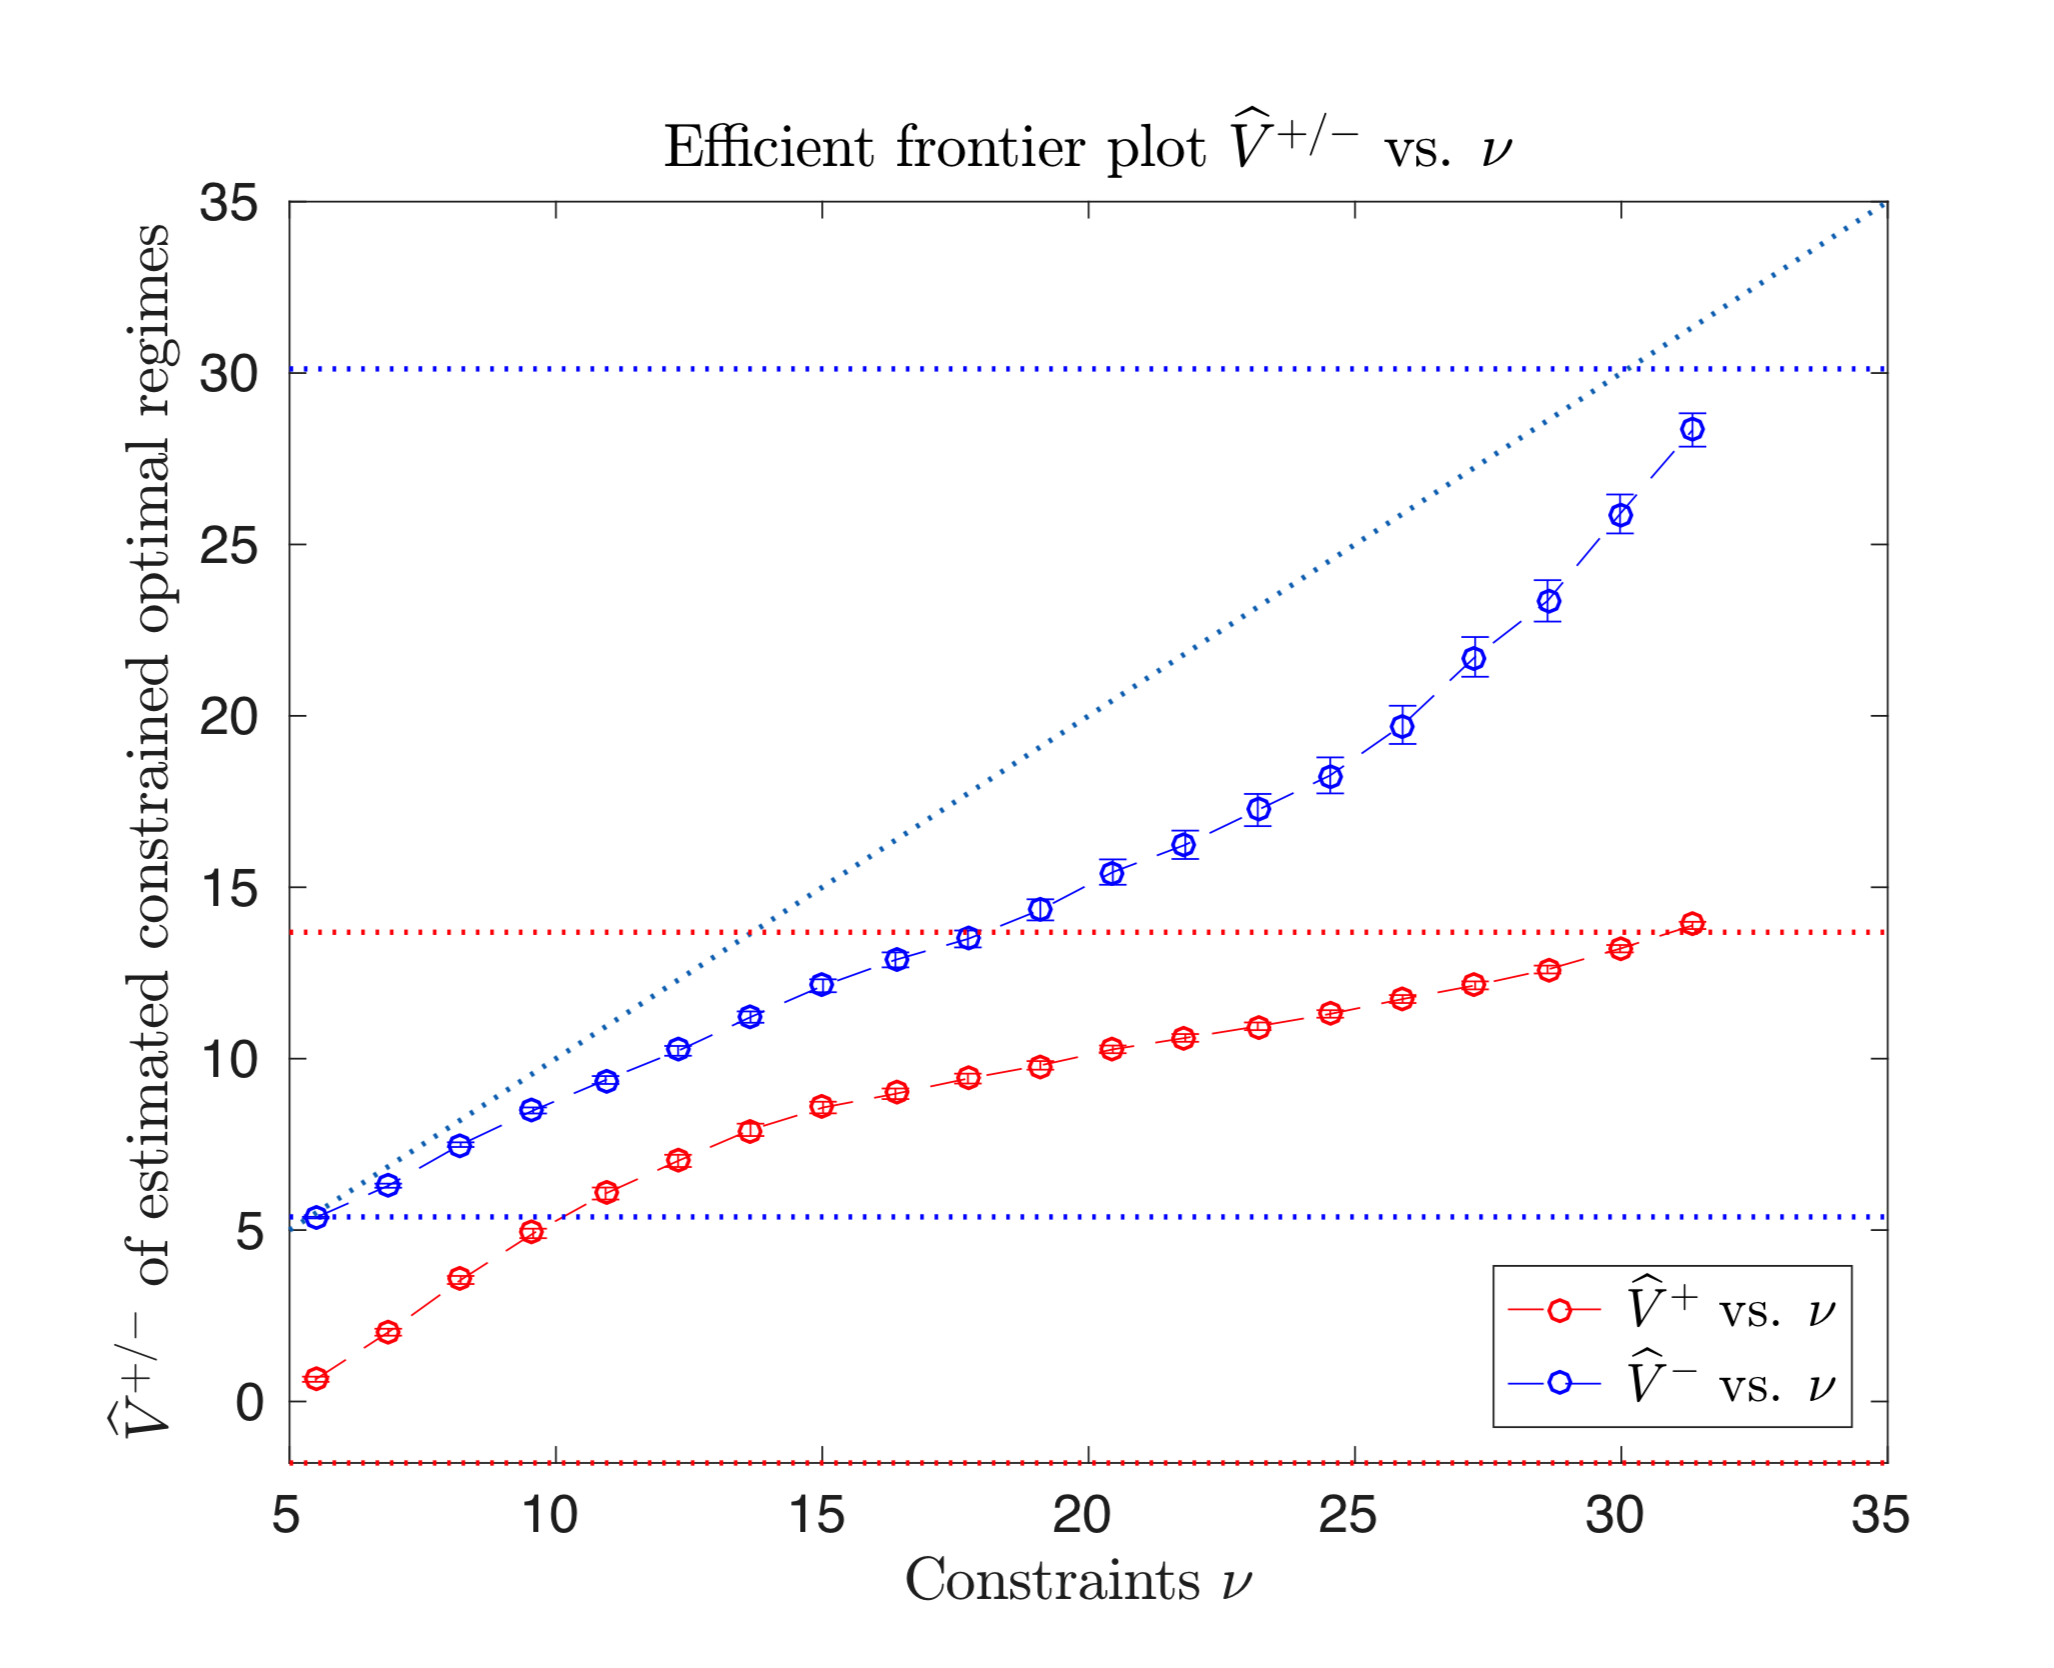
\includegraphics[width=.9\linewidth]{./figs/efficient_plot.png}
	\caption{Efficient frontier for estimated constrained optimal regimes (infinite-stage).}
	\caption*{The red dashed line is for the primary outcome to maximized. The blue dashed line is for the secondary outcome to be constrained. The red dotted lines are the minima and maxima for unconstrained optimization of the primary objective. The blue dotted lines are the minimal and maximal for unconstrained optimization of the secondary objective.}
	\label{fig:1}
\end{figure}
%\begin{figure}[!htbp]
%	\centering
%	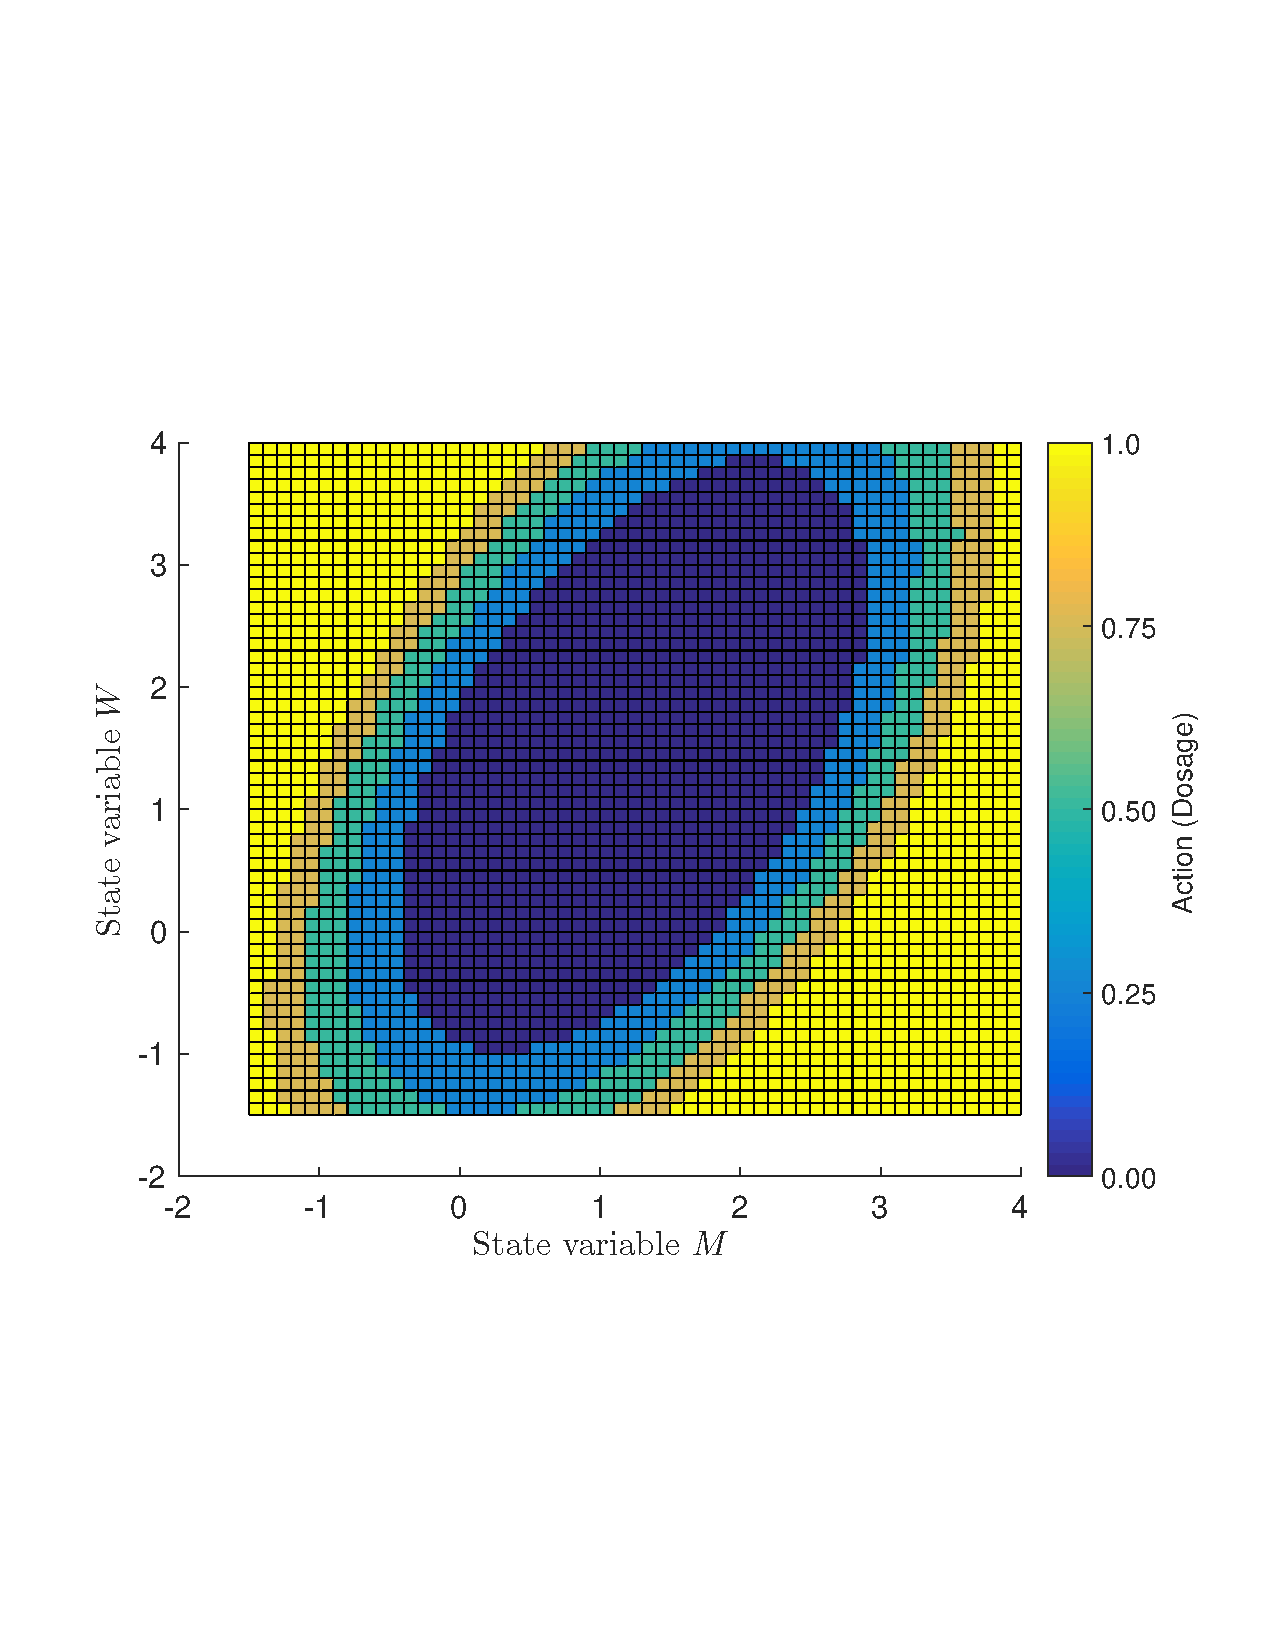
\includegraphics[width=.9\linewidth]{./Chapter-4/figs/action_nu5.pdf}
%	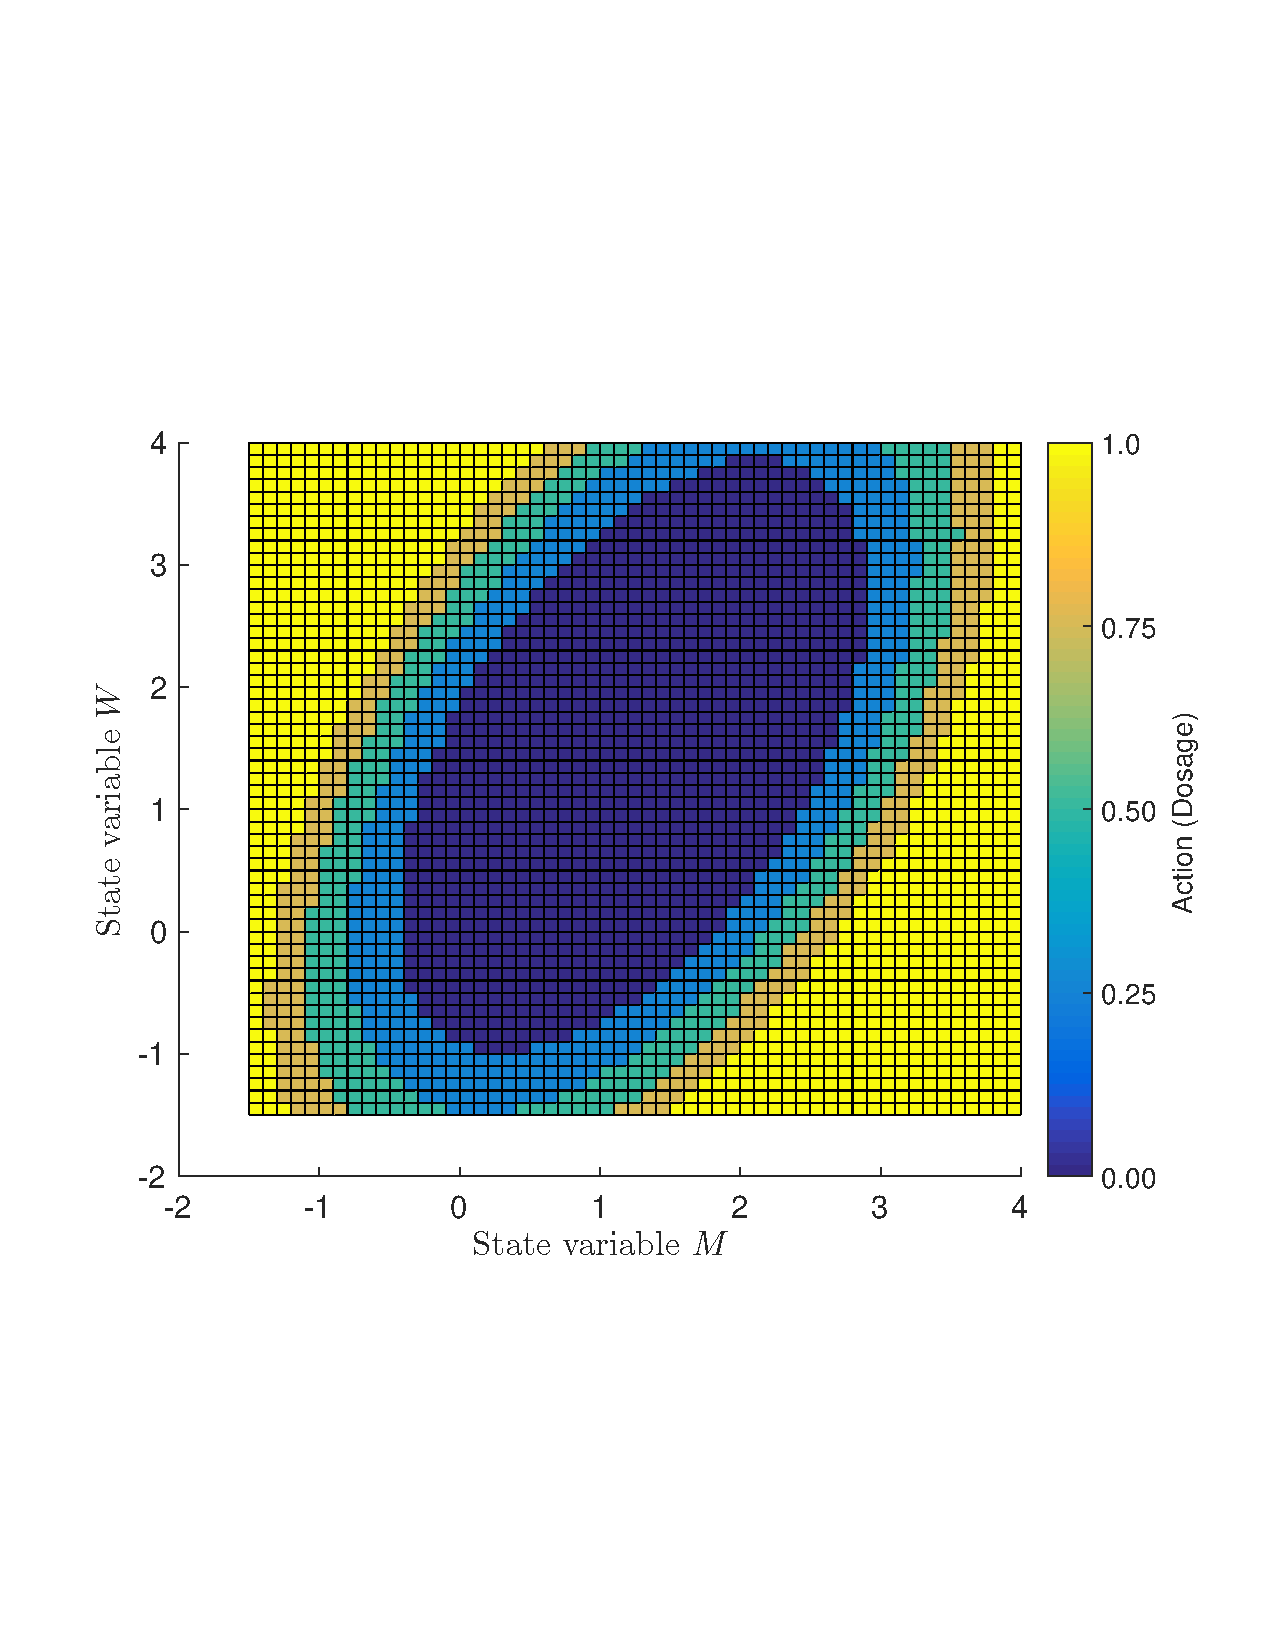
\includegraphics[width=.9\linewidth]{./Chapter-4/figs/action_nu5.pdf}
%	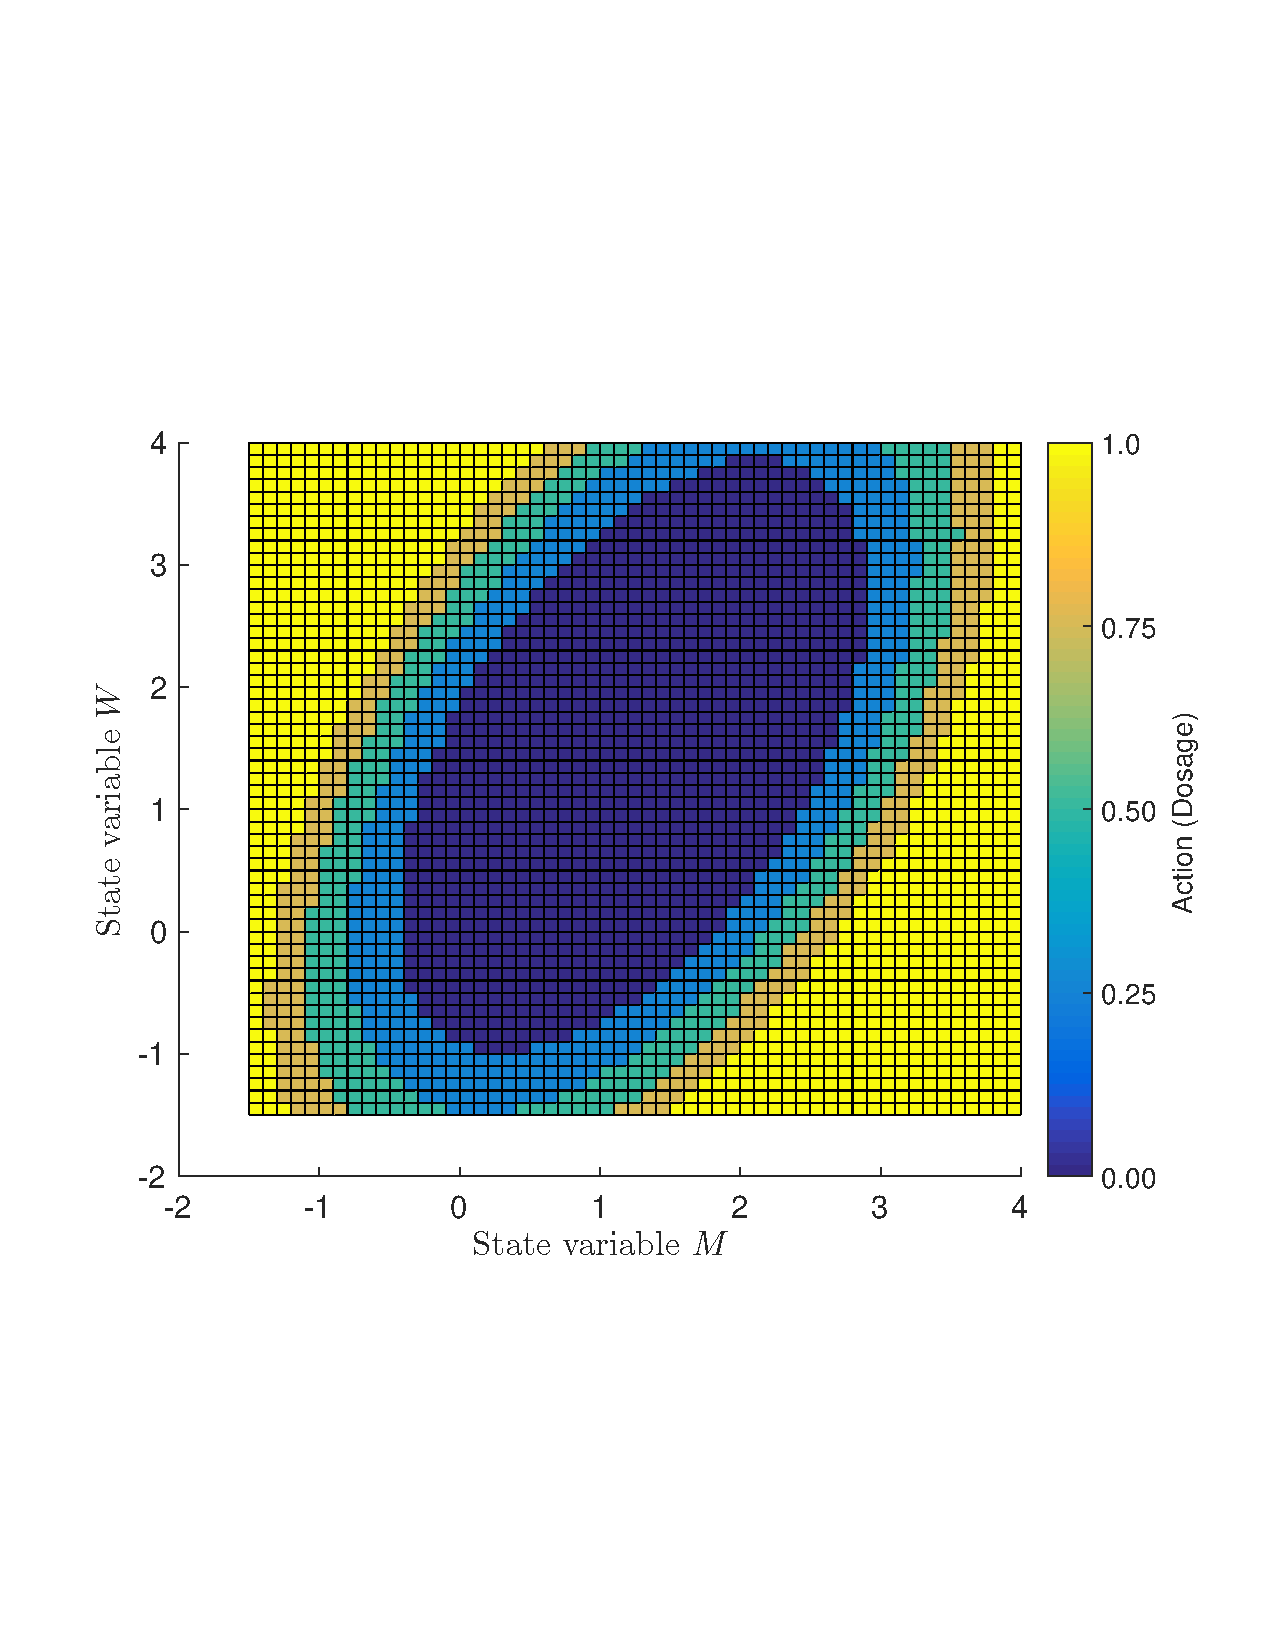
\includegraphics[width=.9\linewidth]{./Chapter-4/figs/action_nu5.pdf}
%	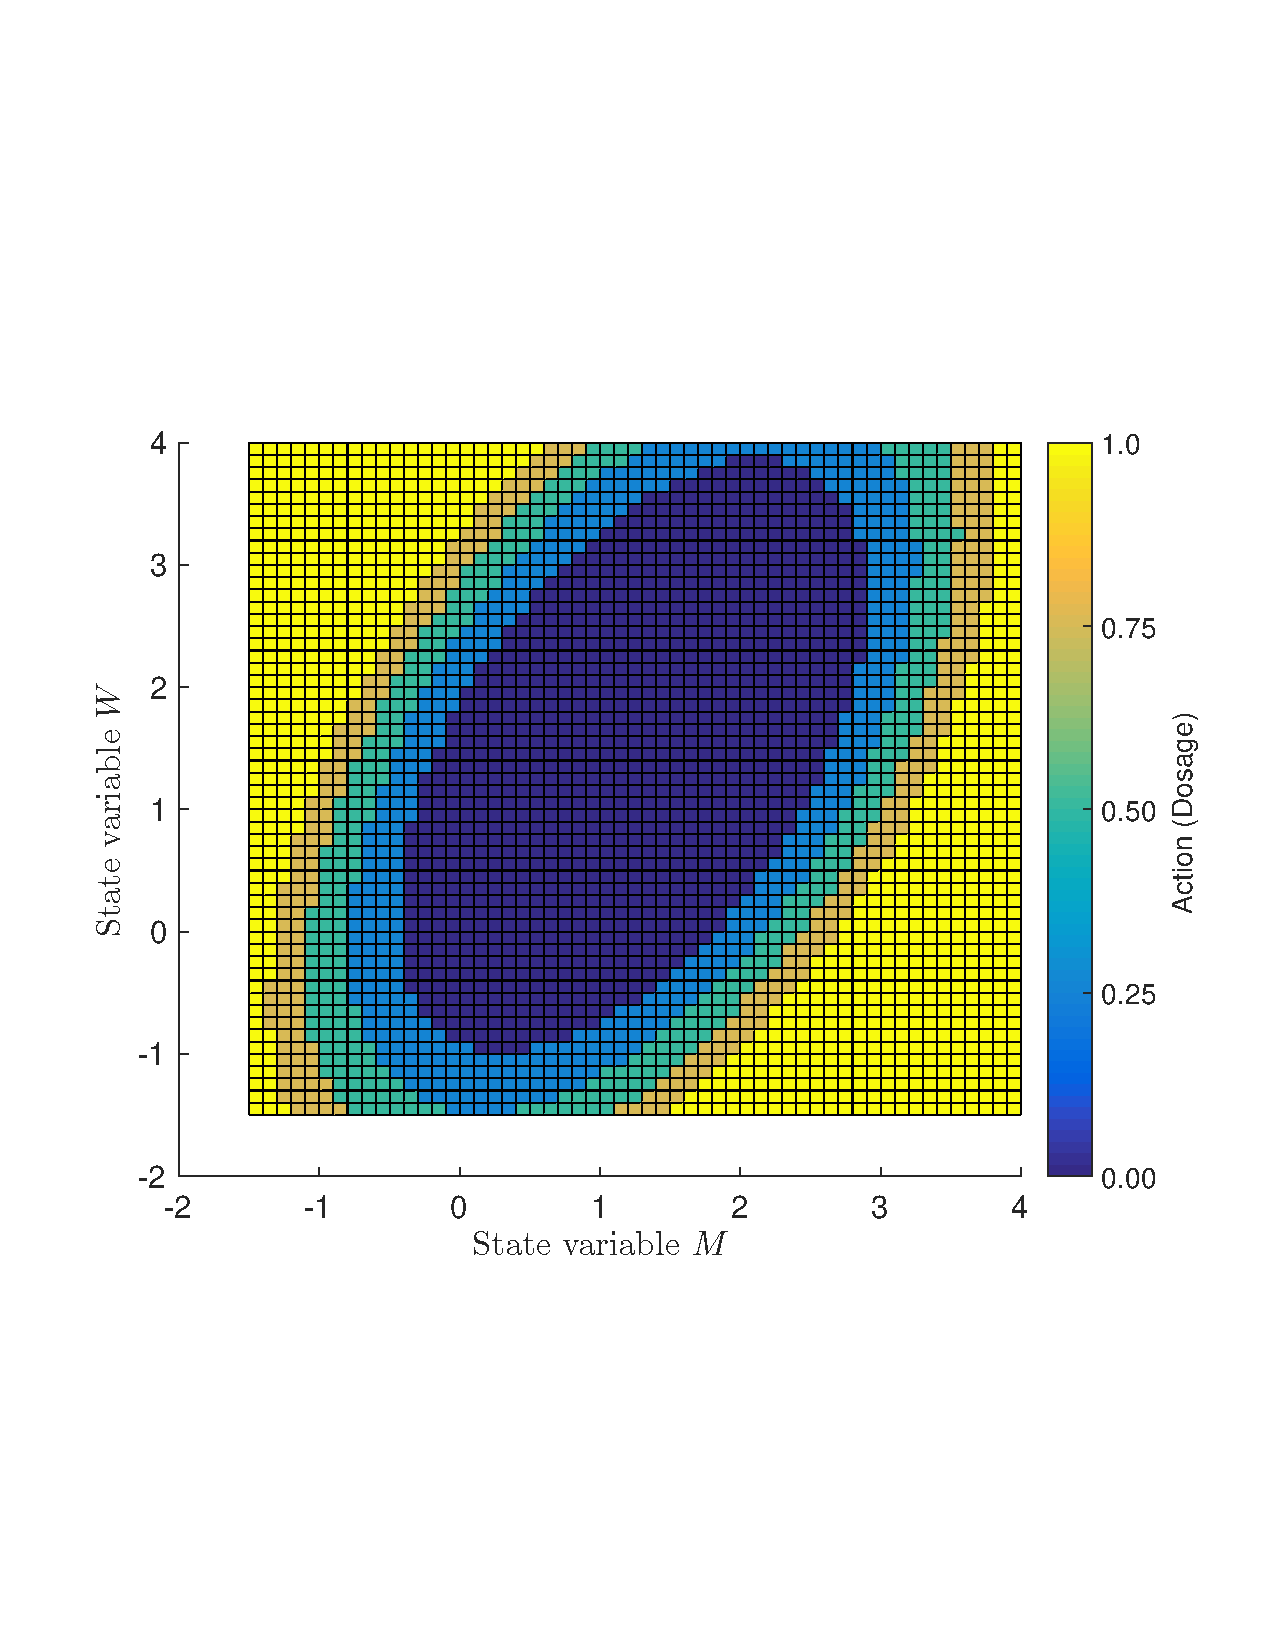
\includegraphics[width=.9\linewidth]{./Chapter-4/figs/action_nu5.pdf}
%	\caption{Action for each state under constraint bounds $\nu$}
%	\caption*{The red dotted line is for the primary outcome to maximized. The blue dotted line is for the secondary outcome to be constrained.}
%	\label{fig:1}
%\end{figure}
%\begin{minipage}{\linewidth}
%	\centering
	\begin{minipage}{0.95\linewidth}
		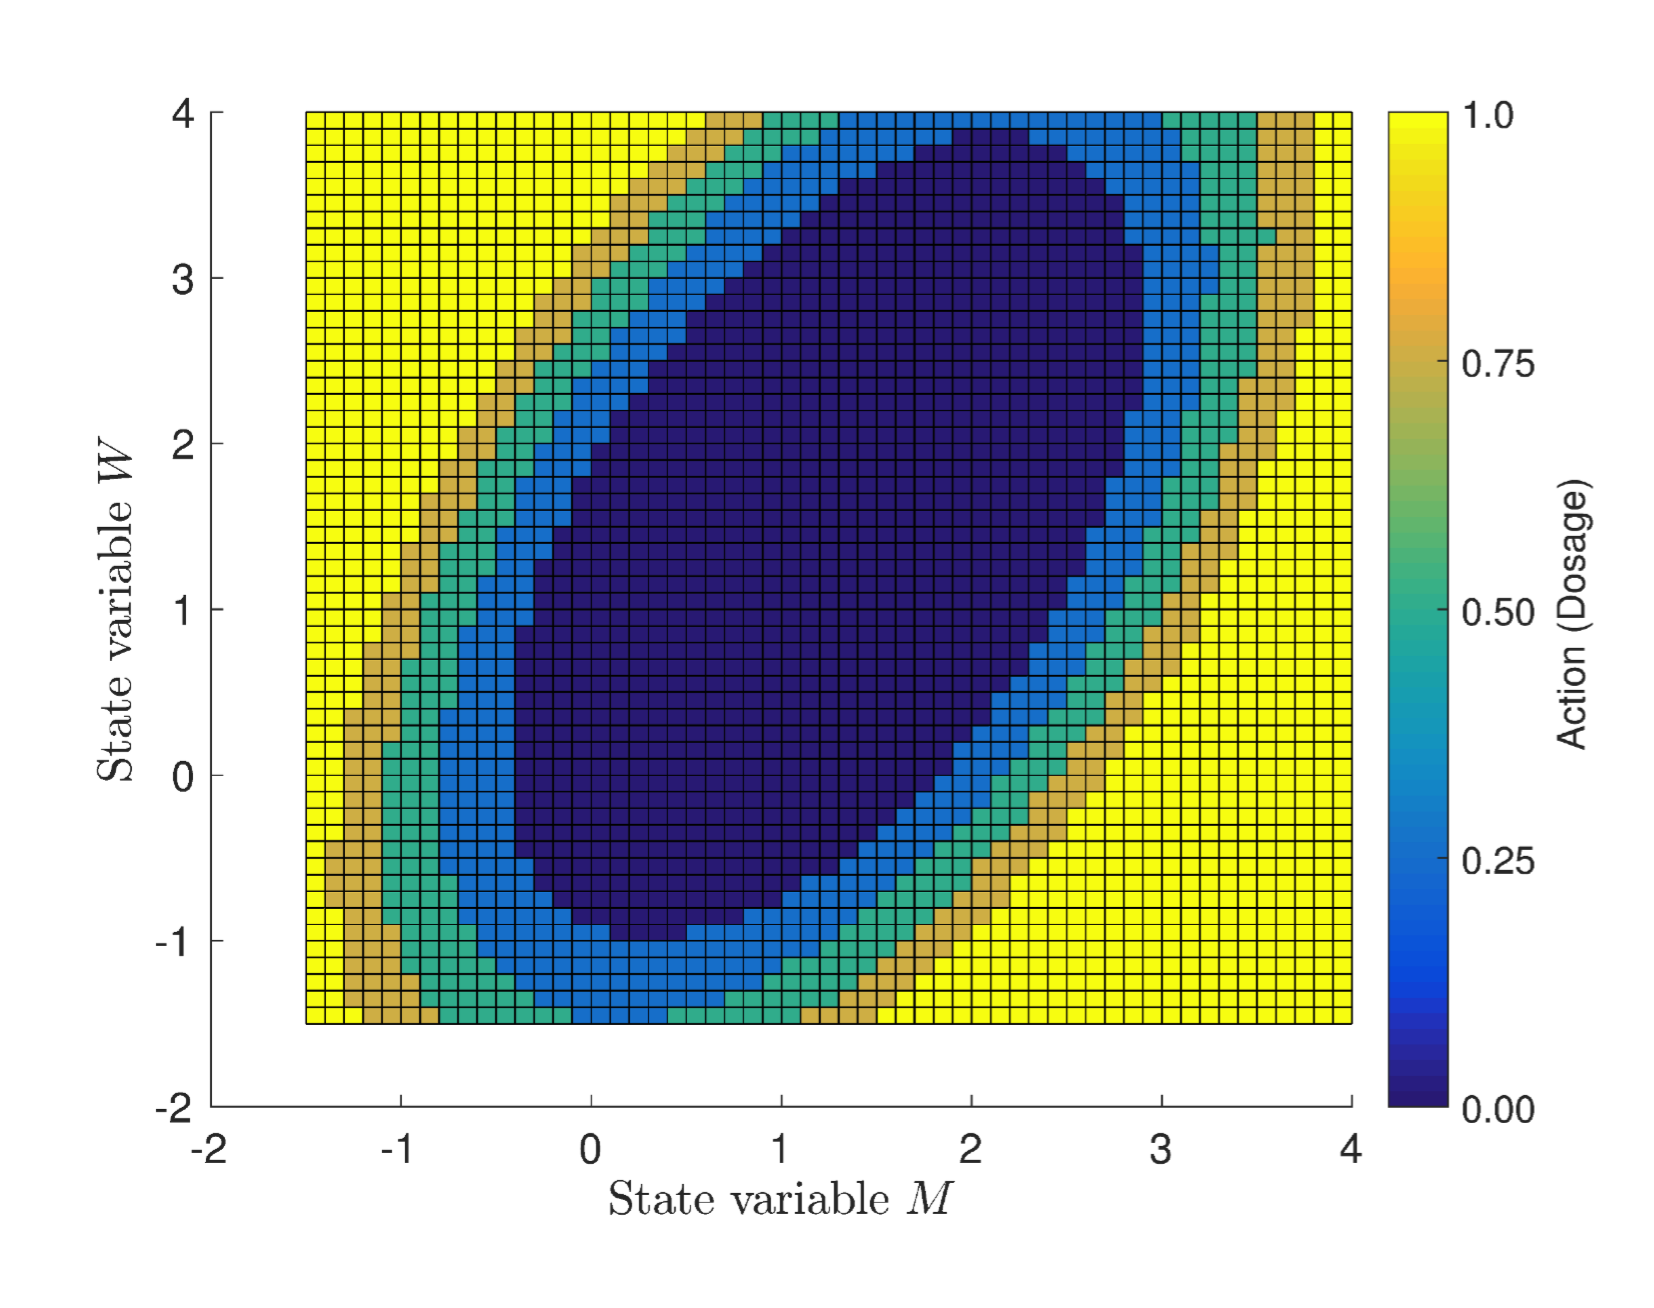
\includegraphics[width=\linewidth]{./figs/action_nu5.png}
		\captionof{figure}{ Action for each state under constraint $\nu=10.93$}
		\caption*{Yellow represents high dosage treatment assignment. Blue represents low dosage assignment. As the constraint bound gets loose, more higher dosage treatments are assigned to patients.}
	\end{minipage}
	\newpage
	\begin{minipage}{0.95\linewidth}
		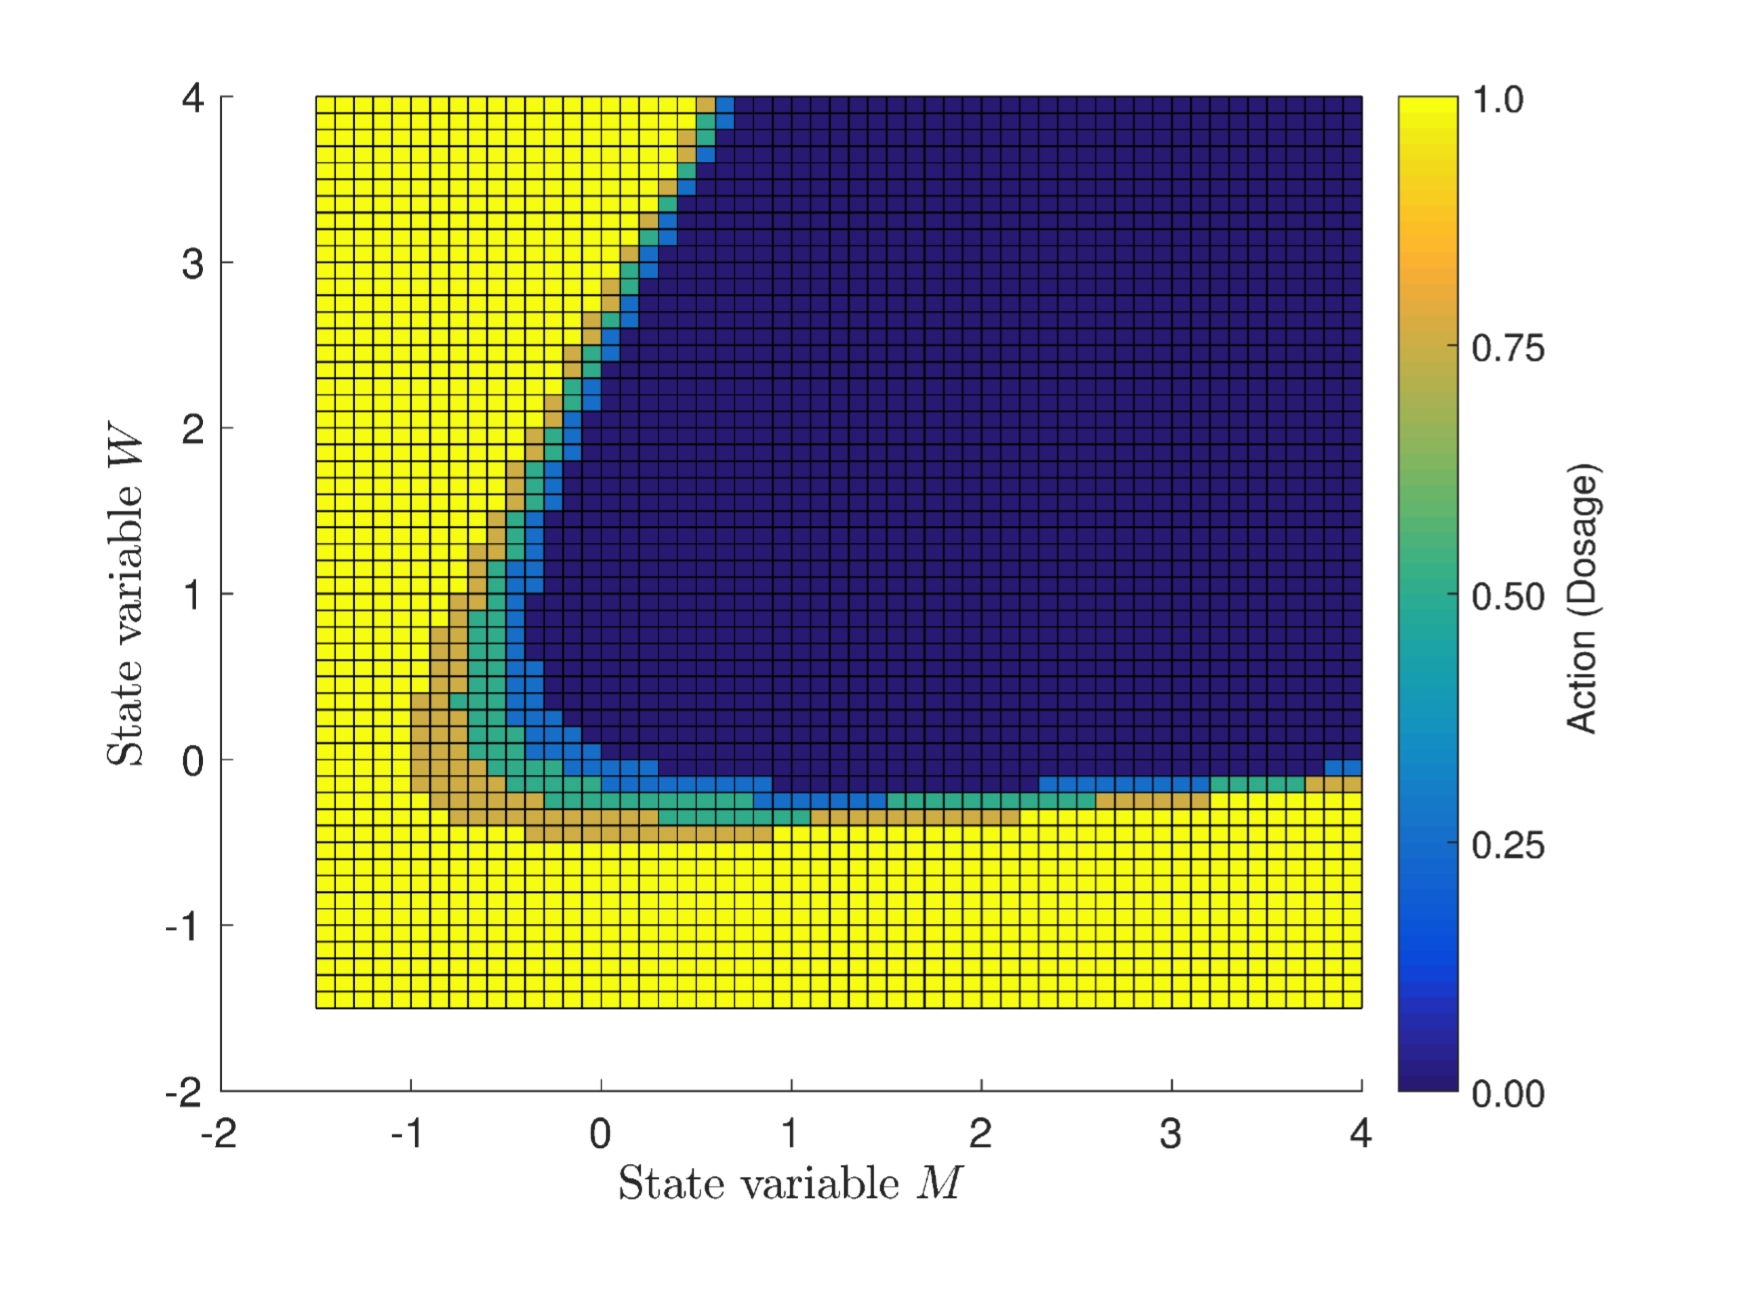
\includegraphics[width=\linewidth]{./figs/action_nu10.png}
		\captionof{figure}{Action for each state under constraint $\nu=17.73$}
		\caption*{Yellow represents high dosage treatment assignment. Blue represents low dosage assignment. As the constraint bound gets loose, more higher dosage treatments are assigned to patients.}
	\end{minipage}
		\newpage
	\begin{minipage}{0.95\linewidth}
		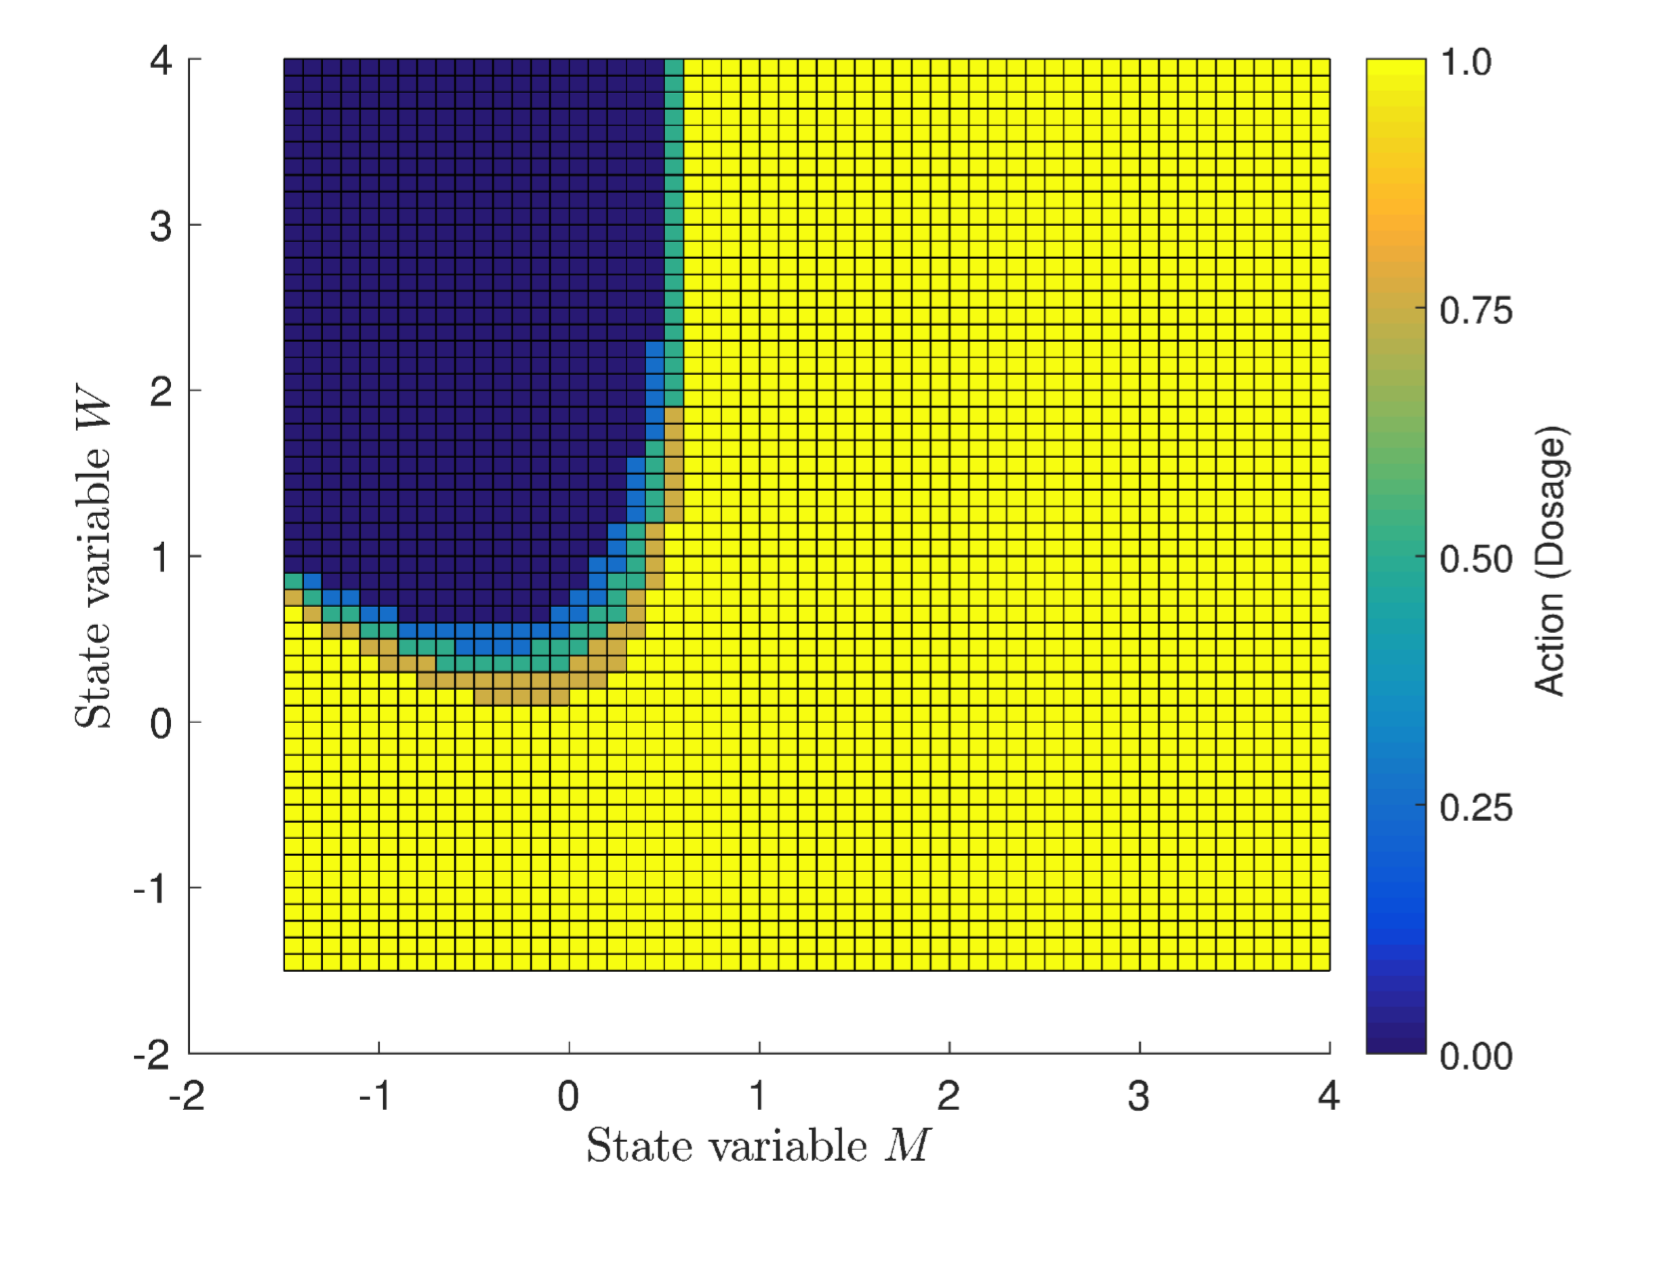
\includegraphics[width=\linewidth]{./figs/action_nu15.png}
		\captionof{figure}{Action for each state under constraint $\nu= 24.54$}
		\caption*{Yellow represents high dosage treatment assignment. Blue represents low dosage assignment. As the constraint bound gets loose, more higher dosage treatments are assigned to patients.}
	\end{minipage}
		\newpage
	\begin{minipage}{0.95\linewidth}
		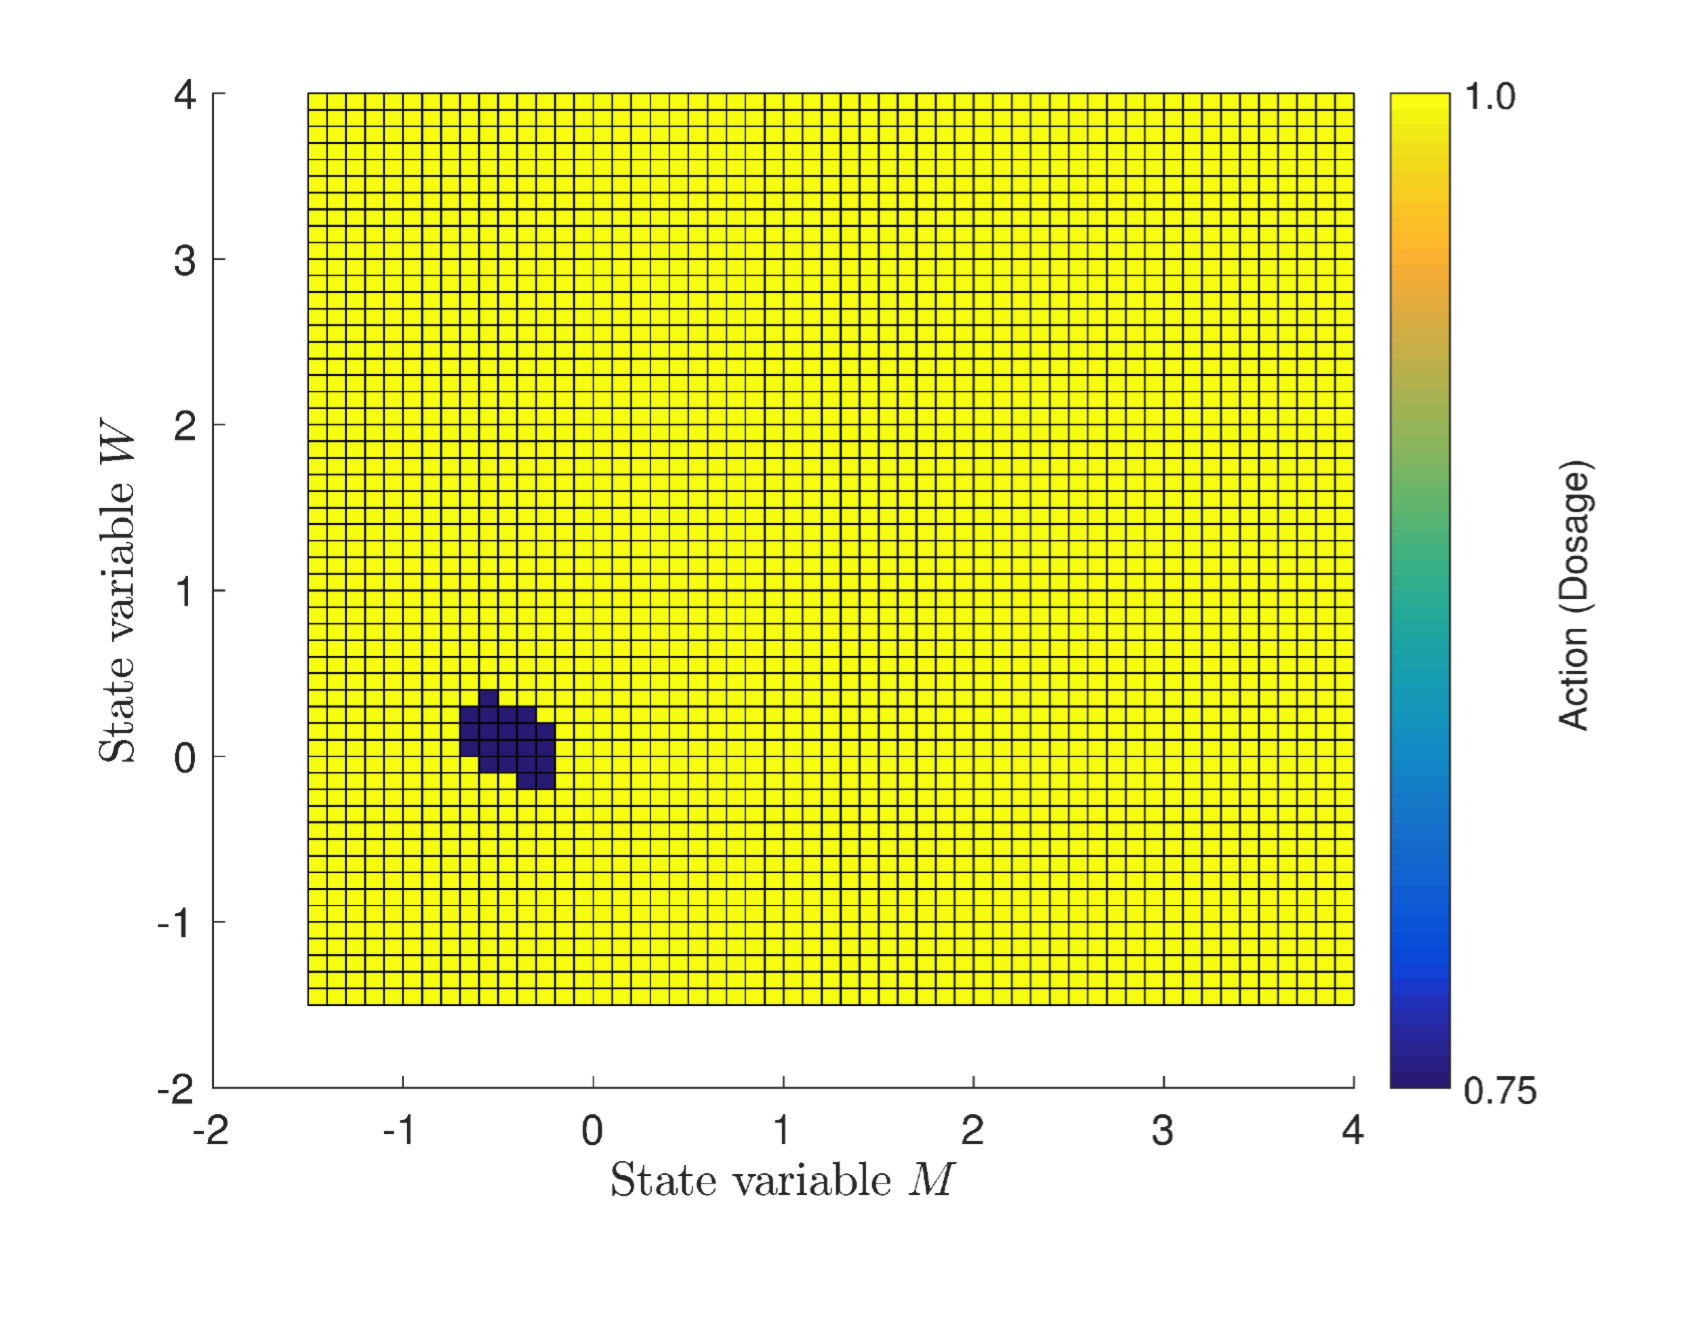
\includegraphics[width=\linewidth]{./figs/action_nu20.png}
		\captionof{figure}{Action for each state under constraint $\nu=31.34$}
		\caption*{Yellow represents high dosage treatment assignment. Blue represents low dosage assignment. As the constraint bound gets loose, more higher dosage treatments are assigned to patients.}
	\end{minipage}
%\end{minipage}
\section{Conclusion and Future}
We propose a framework for constrained optimal dynamic treatment regimes to handle the trade-off between the primary objective and all other secondary objectives in infinite stage setting. The simulation results based on the chemotherapy ODE system are presented and visualized. This framework offers an intuitive way for clinicians to exam the trade-off and make treatment decisions based on patient's preference. Different from CPO, our method takes into consideration that clinical data is expensive and scarce. Borrowing strength from least-squares policy evaluation, our method is able to learn from data efficiently. Moreover, least-squares policy evaluation is an iterative method for policy evaluation, and has the advantage of being able to learn both offline and online. Hence, our method can fits in not only the situation where clinical policies needed to be learned after data collect (offline, off-policy batched), but also the situation where online real-time policy learning is needed. Interior-point method is also a well-studies optimization method for constrained estimation. Its theoretical guarantees assure us of good enough optimal solutions. However, it is obvious that the choice of policy function approximation may have impact on the decision. So does the choice of Q function approximation. Clinical domain expertise may required. Alternatively, automated feature learning techniques for function approximation from the machine learning community can be incorporated. More complex dataset maybe collected, such as text, image, speech and so on, considering the recent technology advancement in mobile devices. How to incorporate those complex information to better describe an individual's state of health is challenging. Rigorous theoretical work for our method is also under investigation.\\

Besides constraints on the expected value of a policy, we can also consider risk constraints, where the probabilities of adverse events occurring are restricted. Although reinforcement learning is a powerful technique to find optimal treatment regimes for clinical practice, designing appropriate reward functions is crucial for serving the desired clinical purpose, but very difficult. Current approach may not scale well in complex clinical situations or preventive healthcare where multiple subgoals may be involved. How to automatic generate rewards and objectives in complex clinical situations can be an interesting direction for investigation.\\

Nowadays, many aspects of the clinical practice have been transformed by mobile devices, such as smart phones, tablets, wearable sensors etc. It allows clinicians remotely monitor and intervene patients’ chronic conditions in real-time. It also allows for adaptive preventive interventions for motivating and maintaining healthy behaviors, such as physical exercise, diets, and so on. To better understand adaptive interventions, interdisciplinary collaborations becomes a necessity among clinicians, medical researchers, behavioral scientists, statisticians, and computer scientists.\\

% Preventive healthcare can be a possible application. thods to avoid occurrence of disease either through eliminating disease agents or increasing resistance to disease.[15] Examples include immunization against disease, maintaining a healthy diet and exercise regimen, and avoiding smoking.[16]
 % Rewards signal can be sparse as well. agent to automatically discover the range of tasks that it is capable of performing. We use a generator network to propose tasks for the agent to try to achieve, specified as goal states. The generator network is optimized using adversarial training to produce tasks that are always at the appropriate level of difficulty for the agent. Our method thus automatically produces a curriculum of tasks for the agent to learn. We show that, by using this framework, an agent can efficiently and automatically learn to perform a wide set of tasks without requiring any prior knowledge of its environment. Our method can also learn to achieve tasks with sparse rewards, which traditionally pose significant challenges.

% Automatic Goal Generation for Reinforcement Learning Agents. David Held, Xinyang Geng, Carlos Florensa, Pieter Abbeel

% In this paper, we consider Markov Decision Processes (MDPs) with error states. Error states are those states entering which is undesirable or dangerous. We define the risk with respect to a policy as the probability of entering such a state when the policy is pursued  \\

\bibliography{ShupingR-thesis}{}
\bibliographystyle{plain}
\begin{appendices}
\section{Least-squares policy evaluation (LSQ) algorithm}
\begin{algorithm}[H]
	\caption{LSQ}
	$A \leftarrow 0$ \\
	$b \leftarrow 0$ \\
	for each $(s,a, s^{\prime}, r)$
	
	\hspace{25pt} $A \leftarrow A + \phi(s,a)\lt(\phi(s,a) - \gamma \phi(s',\pi(s')\rt)^\intercal $
	
	\hspace{25pt} $b \leftarrow  b + \phi(s,a)r$
	
	$w	\leftarrow A^{-1}b$
	
	return $w$
\end{algorithm}
	
\end{appendices}

\end{document}